\RequirePackage{rotating}
\documentclass[man,floatsintext,a4paper,biblatex]{apa6}\usepackage[]{graphicx}\usepackage[]{color}
%% maxwidth is the original width if it is less than linewidth
%% otherwise use linewidth (to make sure the graphics do not exceed the margin)
\makeatletter
\def\maxwidth{ %
  \ifdim\Gin@nat@width>\linewidth
    \linewidth
  \else
    \Gin@nat@width
  \fi
}
\makeatother

\definecolor{fgcolor}{rgb}{0.345, 0.345, 0.345}
\newcommand{\hlnum}[1]{\textcolor[rgb]{0.686,0.059,0.569}{#1}}%
\newcommand{\hlstr}[1]{\textcolor[rgb]{0.192,0.494,0.8}{#1}}%
\newcommand{\hlcom}[1]{\textcolor[rgb]{0.678,0.584,0.686}{\textit{#1}}}%
\newcommand{\hlopt}[1]{\textcolor[rgb]{0,0,0}{#1}}%
\newcommand{\hlstd}[1]{\textcolor[rgb]{0.345,0.345,0.345}{#1}}%
\newcommand{\hlkwa}[1]{\textcolor[rgb]{0.161,0.373,0.58}{\textbf{#1}}}%
\newcommand{\hlkwb}[1]{\textcolor[rgb]{0.69,0.353,0.396}{#1}}%
\newcommand{\hlkwc}[1]{\textcolor[rgb]{0.333,0.667,0.333}{#1}}%
\newcommand{\hlkwd}[1]{\textcolor[rgb]{0.737,0.353,0.396}{\textbf{#1}}}%

\usepackage{framed}
\makeatletter
\newenvironment{kframe}{%
 \def\at@end@of@kframe{}%
 \ifinner\ifhmode%
  \def\at@end@of@kframe{\end{minipage}}%
  \begin{minipage}{\columnwidth}%
 \fi\fi%
 \def\FrameCommand##1{\hskip\@totalleftmargin \hskip-\fboxsep
 \colorbox{shadecolor}{##1}\hskip-\fboxsep
     % There is no \\@totalrightmargin, so:
     \hskip-\linewidth \hskip-\@totalleftmargin \hskip\columnwidth}%
 \MakeFramed {\advance\hsize-\width
   \@totalleftmargin\z@ \linewidth\hsize
   \@setminipage}}%
 {\par\unskip\endMakeFramed%
 \at@end@of@kframe}
\makeatother

\definecolor{shadecolor}{rgb}{.97, .97, .97}
\definecolor{messagecolor}{rgb}{0, 0, 0}
\definecolor{warningcolor}{rgb}{1, 0, 1}
\definecolor{errorcolor}{rgb}{1, 0, 0}
\newenvironment{knitrout}{}{} % an empty environment to be redefined in TeX

\usepackage{alltt}
\usepackage[english, british]{babel}
\usepackage[style=apa,sortcites=true,sorting=nyt,backend=biber]{biblatex}
\DeclareLanguageMapping{british}{british-apa}
% http://tex.stackexchange.com/questions/162212/initials-in-the-bibliography-firstinits-uniquename-not-working-correctly-in-bib
\DeclareSourcemap{
  \maps[datatype=bibtex]{
    \map{
       \step[fieldsource=sortname]
       \step[fieldset=namea, origfieldval, final]
    }
  }
}
\DeclareLabelname{
  \field{namea}
  \field{shortauthor}
  \field{author}
  \field{shorteditor}
  \field{editor}
  \field{translator}
}
\addbibresource{bibliography.bib}
\usepackage[utf8]{inputenc}
\usepackage[T1]{fontenc}
\usepackage{amsmath}
\usepackage{amssymb,amsfonts,textcomp}
\usepackage{array}
\usepackage{hhline}
\usepackage{graphicx}
\usepackage[page,header]{appendix}
\usepackage{titletoc}
\usepackage{lipsum}

\usepackage[]{hyperref}
\hypersetup{
    bookmarksnumbered=true,     
    bookmarksopen=true,         
    bookmarksopenlevel=1,       
    colorlinks=true,            
    allcolors=blue,
    pdfstartview=Fit,           
    pdfpagemode=UseOutlines,    % this is the option you were lookin for
    pdfpagelayout=TwoPageRight
}
\usepackage{cleveref}
\usepackage[table]{xcolor}
\usepackage[textwidth=2cm,color=green,textsize=tiny]{todonotes}
\reversemarginpar
\usepackage{afterpage}
\makeatletter
\newcommand\arraybslash{\let\\\@arraycr}
\makeatother
\setlength\tabcolsep{1mm}
\renewcommand\arraystretch{1.3}
\newcounter{Figure}
\renewcommand\theFigure{\arabic{Figure}}

%\fancyhead{}
%\fancyfoot{}
\renewcommand{\headrulewidth}{0pt}
%\fancyhead[RO,LE]{\footnotesize\thepage}
\fancyhead[CO,CE]{\footnotesize EFFECTS OF ABM ON RUMINATION AND WORRY ABOUT CURRENT CONCERNS}
%\fancyhead[RE]{\footnotesize\slshape\leftmark}
%\pagestyle{fancy}

\title{The effects of attentional bias modification on rumination and worry about current concerns: a case-series}
\shorttitle{}
\author{Paul Sharpe}
\affiliation{University of Exeter}
\note{Word count: 7966}
\leftheader{Attentional bias modification of rumination towards a self-relevant goal: A case-series}

\abstract{Rumination and worry are thinking styles closely associated
with depression and anxiety, and there is evidence to suggest that
an attentional bias towards negative stimuli plays a role in these
associations. A hypothesis arising from the attentional bias literature is
that depressive rumination results from an impaired ability to disengage
attention from self-referent negative thoughts, and that reducing this
bias will reduce rumination and depressive symptoms. A broader theory
proposes that rumination is the result of discrepancies between perceived
and expected progress towards goals. Current concerns are mental states
representative of such goal progress discrepancies. The current study
tests the disengagement hypothesis within this goal progress theory
of rumination. It aims to reduce attentional bias to towards negative
words and words associated with an unresolved current concern, and
detect corresponding reductions in rumination, worry, mood and symptoms
of anxiety and depression. Participants were 12 (10 female) university
students or staff scoring low for depressive symptoms but high for trait
rumination and/or trait worry. Attentional bias was measured using a
dot-probe task. Attentional bias modification training (ABMT) consisted
of a modified dot-probe task. Stimuli were negative--neutral word pairs,
and neutral words paired with words associated with a current concern
chosen by each participant. Using a multiple baseline case-series design,
each participant completed between 25--35 dot-probe sessions at home,
a minimum of 8 sessions also included ABMT. There were no significant
post-training effects on trait rumination, trait worry, and symptoms of
depression and anxiety. Randomisation tests showed no significant post
ABM reduction in attentional bias towards negative words, attentional
bias towards current concern words, rumination towards the concern,
positive affect, negative affect or depressive symptoms. The limitations
of the dot-probe task are discussed and the cost-effectiveness of ABMT
as psychological therapy evaluated.}

\authornote{I would like to acknowledge the continuous support provided by
Nick Moberly in supervising this research, and for advice on randomisation
tests within case-series designs provided by Patrick Onghena and Stephen
Morley.}

% http://tex.stackexchange.com/questions/35532/using-newcommand-in-includegraphics-option-to-substitute-graphic-sizes
\makeatletter
\define@key{Gin}{plotwh}[true]{%
    \edef\@tempa{{Gin}{width=90mm,height=70mm}}%
    \expandafter\setkeys\@tempa
}
\makeatother

\usepackage{amsmath,siunitx,caption}
\newcommand{\IE}[1][1]{% indent entry
  \hspace{#1em}\ignorespaces
}
\usepackage{mathtools}
\usepackage{csvsimple}

\usepackage{pifont}
\usepackage{booktabs}
\newcommand*\rot{\rotatebox{90}}

\usepackage{tabularx}
\usepackage{tikz}
\newcommand\strokeA{\tikz[baseline=-.5ex]{ \draw[black,thick,align=center] (0,0) -- (2ex,0); }}
\newcommand\strokeB{\tikz[baseline=-.5ex]{ \draw[red,thick,dotted] (0,0) -- (2ex,0); }}
\newcommand\strokeC{\tikz[baseline=-.5ex]{ \draw[black,thick,dotted] (0,0) -- (2ex,0); }}

\usepackage{subcaption}

% Dilemma, doing this gets cref working for sections but adds section numbers which breaks APA
%\setcounter{secnumdepth}{3}

% Nick says no issue number or month for APA
\AtEveryBibitem{%
%  \ifboolexpr{test {\ifentrytype{article}} and not test {\iffieldundef{doi}}}
  \ifboolexpr{test {\ifentrytype{article}}}
    {
      \clearfield{number}
      \clearfield{month}
      \clearfield{note}
    }
    {}%
}
\IfFileExists{upquote.sty}{\usepackage{upquote}}{}
\begin{document}\thispagestyle{empty}
\setlength{\marginparwidth}{1cm}
%\todototoc
%\listoftodos[Todo list]
\maketitle
\pdfbookmark{\contentsname}{toc}
%\tableofcontents
\startcontents[sections]
\printcontents[sections]{l}{1}{\setcounter{tocdepth}{2}}
\newpage

\section{Introduction}
\label{introduction}

Anxiety and depression are major challenges to public health and
are commonly co-morbid \parencite{kessler_impairment_1999},
with mixed depression and anxiety were reported as being
present in 9.0\% of English adults in the most recent household
survey \parencite{mcmanus_adult_2009}. Whilst this reflects
a level of stability in prevalence over the preceding 7 years,
\textcite{mathers_projections_2006} project that in 2030 unipolar
depression will be the second most common cause of disability-adjusted
life years. Based on 2007 prevalence rates, \textcite{mccrone_paying_2008}
estimate that the combined cost of depression and anxiety services
in England in 2026 will be \pounds5 billion, with lost employment
bringing the total cost to \pounds26.4 billion. To address these
issues, \textcite{mccrone_paying_2008} recommend expanding provision of
evidence-based interventions in primary care settings with a focus on
the most cost-effective means of delivery, such as Internet delivered
cognitive behavioural therapy (I-CBT).

Despite their strong evidence-base, pharmacological and psychological
treatments are only partially effective. Combinations of these
treatments are effective at treating depression in about 33\%  of
cases \parencite{andrews_utilising_2004}, and CBT, the gold standard
psychological treatments, has response rates of 50\% or less for
treating anxiety disorders \parencite{schneider_state_2015}. In
England in May 2015, 96.1\% people referred for a course of
psychological therapy waited less than 18 weeks for treatment
\parencite{hsiccommunityandmentalhealthteam_improving_2015}, which is an
improvement on the British average waiting times of six to nine months
in 2007 \parencite{haliwell_fundamental_2007}. However, there are
high costs associated with delivering psychological therapies and some
evidence that the efficacy of CBT for treating depression is falling
\parencite{johnsen_effects_2015}.

% handle weird gaps that appeared between paragraphs near this page
\raggedbottom

Technological advances may improve cost-effective treatment
delivery. I-CBT is a viable treatment for adults with depression and
some anxiety disorders \parencite{arnberg_internetdelivered_2014},
and mobile apps including real-time monitoring of mood and behaviour
could also contribute \parencite{cuijpers_psychotherapies_2015}. More
research is required to ascertain whether this potential can be realised
in practice.  An expanded understanding of the role played by cognitive
mechanisms such as attention and memory in mood disorders is reflected
in the greater precision of newer treatments. For example, Mindfulness
Based Cognitive Therapy (MBCT) is a treatment which specifically
targets depressive relapse \parencite{segal_mindfulnessbased_2012},
which is common and becomes increasingly likely with each depressive
episode \parencite{haliwell_fundamental_2007}. The most effective new
treatments for depression and anxiety are likely to draw on evidence
which explicates the role that cognitive mechanisms play in these common
disorders, and computer tasks offer one cost-effective means of delivery.

Rumination is a repetitive thinking style closely linked to depression
and anxiety, which in turn are associated with psychological distress and
physical health difficulties. A more precise definition of rumination
distinguishes unconstructive repetitive thoughts associated with
depression and anxiety, from more constructive forms of repetitive
thought which support planning, problem solving, and healthy
self-reflection \parencite{watkins_constructive_2008}.  Whilst there
is broad consensus regarding the role played by rumination, the ten
models and five measures reviewed by \textcite{smith_roadmap_2009}
demonstrate that ``there is no unified definition [...] or standard way
of measuring it'' \textcite[][p. 117]{smith_roadmap_2009}. Response
styles theory \parencite[RST; ][]{nolen-hoeksema_responses_1991}
considers rumination to be a particular response to depressed mood
where a person tends to focus on ``causes, consequences and symptoms
of one's negative affect'' \parencite[][p. 117]{smith_roadmap_2009}
thereby prolonging low mood and depressive episodes. The Ruminative
Responses Scale (RRS) \parencite{treynor_rumination_2003}, derived
from RST, is considered the gold standard trait measure of rumination,
containing sub scales which can distinguish maladaptive rumination in
the form of 'depressive brooding' from the more adaptive 'reflective
pondering'. In support of RST, dysphoric mood is significantly
increased by a rumination induction and significantly decreased by a
distraction induction, in dysphoric but not in non-dysphoric participants
\parencite{nolen-hoeksema_rethinking_2008}.  However, the positive effects
of distraction are temporary \parencite{nolen-hoeksema_rethinking_2008},
and alternative models of rumination may suggest more effective ways to
reduce its occurrence.

The goal progress theory of rumination \parencite{martin_ruminative_1996}
is one such model, which proposes that rumination is initiated
by unexpected progress (more or less) towards a goal\footnote{An
extension of the model draws on parallel distributed processing
to explain discrepancies arising amongst ${concurrent}$ goals
\parencite{martin_extending_2006}.}. This account draws on ideas
from control theory \parencite{carver_control_1982} in that
goal discrepancies represent system states outside of desirable
thresholds which cognitive process try to restore through feedback
mechanisms. Rumination is in essence this deployment of attention, memory
and consciousness, and will remain present until goal progress becomes
satisfactory, the goal is perceived as being met, or is abandoned. For
\textcite[][p. 7]{martin_ruminative_1996}, rumination is "a class of
conscious thoughts that revolve around a common instrumental theme and
that recur in the absence of immediate environmental demands requiring
the thoughts". A concept closely related to unresolved goals is the
`current concern', which \textcite[][p.14]{klinger_motivation_2011}
define as \enquote{the state of an individual between the two time points
of becoming committed to pursuing a particular goal and either attaining
it or giving it up}. Current concerns link goal progress to rumination
in that they increase an individual's sensitivity to \enquote{notice,
recall, think about, dream about and act on cues associated with the
goal pursuit} \parencite[][p.2]{klinger_motivation_2011}. Similarly,
negative affect draws attention towrads unsatisfactory goal progress
\parencite{martin_ruminative_1996}.

Worry is a thought process with both similarities and differences to
rumination. \textcite[][p. 10]{borkovec_preliminary_1983} define worry
as \enquote{a chain of thoughts and images, negatively affect-laden and
relatively uncontrollable}. Whilst some studies associate depression
with rumination and worry with anxiety, measures of rumination and worry
are highly correlated \parencite{smith_roadmap_2009}. One distinction
is the prevalence of past events in ruminative thought content,
and the contrasting dominance of future events in the case of worry
\parencite{papageorgiou_depressive_2004,watkins_comparisons_2005}.
\textcite{mclaughlin_effects_2007} supported this general distinction,
however they also found that induced rumination began as past-focused
before displaying a linear trend towards thoughts about the present and
finally the future. Whilst rumination is linked to depression levels
and predicts the onset of depressive episodes, it also predicts
symptoms of anxiety \parencite{nolen-hoeksema_role_2000}. Both
forms of repetitive negative thought regularly occur in the same
individual, suggesting a common underlying processes (at least in
non-clinical populations) \parencite{watkins_comparisons_2005}, and
is consistent with the common co-morbidity of anxiety and depression
\parencite{kessler_impairment_1999}. Studies which have directly compared
rumination and worry point towards similar cognitive impairments, such as
reduced cognitive control \parencite{beckwe_worrying_2014}. In summary,
the content of worrisome and ruminative thoughts may differ, but may
result from similar cognitive processes.

The mechanisms underlying rumination are less well understood than their
affective consequences \parencite{koster_understanding_2011}. For example,
it remains unclear whether rumination is an automatic or consciously
controlled process \parencite{smith_roadmap_2009}. Nevertheless,
numerous studies indicate that a range of cognitive deficits
associated with anxiety and depression may also play a role
in rumination. These include biases of attention, memory,
interpretation and emotional association, and inhibitory control
deficits \parencite{mathews_cognitive_2005}. Attentional bias is a
disproportionate attentional sensitivity to particular stimuli, be they
internal thoughts or external cues \parencite{williams_cognitive_1997},
and one unresolved hypothesis is whether depressive rumination is caused,
at least in part, by an impaired ability to disengage attention from
negative thoughts \parencite{koster_understanding_2011}. Disruption
in attention-focusing ability is also a cognitive correlate
of worry \parencite{borkovec_preliminary_1983}. The causal
direction between rumination and attentional bias is also unclear
\parencite{koster_understanding_2011}. \textcite{morrison_role_2008}
showed that negative mood combined with a rumination induction
decreased bias towards positive word stimuli, whereas a distraction
induction increased this bias. However, these inductions found no
such causal relationship between rumination and decreased bias towards
negative words, the relationship required to support the disengagement
hypothesis. Other studies do indicate this reciprocal causal link between
negative attentional bias and rumination. In a double-blind, randomised
controlled with individuals having mild to severe depressive symptoms,
\textcite{yang_attention_2015} demonstrated that reducing attentional
bias towards sad words led to reductions in rumination and depressive
symptoms, and that the reductions in depressive symptoms was mediated
by reduced rumination.

If cognitive biases underlie emotional disorders,
then cognitive bias modification (CBM) offers potential
treatments \parencite{hertel_cognitive_2011}. The dot-probe task
\parencite{macleod_attentional_1986} is the gold-standard measure of
attentional bias, using differences in response times to visual stimuli
having differing affective valence, such as negative and neutral word
pairs. Participants respond to a probe which appears at one or the
other location of the previously displayed stimuli.  The dot-probe has
two advantages over variants of the Stroop task, in which response time
differences are considered to represent interference between naming a
word's colour, and affective or cognitive bias resulting from reading the
word. First, concurrent presentation (colour and word) in the Stroop makes
it unclear whether competition is between attention or response selection
\parencite{macleod_half_1991}. By temporally separating the stimulus
from the probe, the dot-probe may be a more pure measure of attentional
bias. Second, the dot-probe is easily adapted to modify attentional bias,
by manipulating the probe location to train attention towards, or away
from particular stimuli. Numerous studies have indicated that attentional
bias modification (ABM) may be an effective treatment for anxiety
\parencite{hakamata_attention_2010} and more recently ABM has been shown
to reduce depressive symptoms \parencite{yang_attention_2015}. Critics
of CBM argue that the effect sizes are too small to be clinically
relevant \parencite{cristea_efficacy_2015}. However, advocates
argue that this critique is based on a meta-analysis which didn't
differentiate ABM from other forms of CBM, didn't focus on a single
psychological dysfunction (anxiety), or didn't analyse studies
which demonstrate both attentional bias change ${and}$ corresponding
symptom change \parencite{macleod_attentional_2015}. In demonstrating
the mediating role of rumination in reducing depressive symptoms,
\textcite{yang_attention_2015} met both of these final criteria.

Previous research examining rumination towards current concerns has used
the emotional Stroop \parencite{williams_cognitive_1997}, a less pure
measure of attentional bias than the dot-probe, and one which is unable to
also modify attentional bias. The current study measures attentional bias
using the dot-probe, before testing the effects of ABM training (ABMT)
designed to reduce vigilance towards negative words, and words associated
with a current concern. This can be considered a test of the attentional
disengagement hypothesis \parencite{koster_understanding_2011},
specifically in relation to the goal progress theory of rumination
\parencite{martin_ruminative_1996}. The study also aims to replicate
and extend the findings of \textcite{yang_attention_2015}, by
testing whether ABM can reduce rumination and depressive symptoms
in a non-clinical sample. Given the various conceptualisations of
rumination, \textcite{smith_roadmap_2009} recommend using multiple outcome
measures. The difficulties in distinguishing rumination from worry, and
the common co-morbidity of anxiety and depression also suggest multiple
measures are appropriate. The current study measures the effects of
ABM on daily rumination and mood, and on measures of rumination, worry,
anxiety and depressive symptoms over longer periods. This novel use of
ABMT offers the potential to offer a personalised, cost-effective
treatment for anxiety and depression. Specific hypotheses were:

\begin{enumerate}

\item Attentional bias towards negative words will reduce after ABMT. 

\item Attentional bias towards ideographic words associated with a
current concern will reduce after ABMT. 

\item Trait worry, rumination over the previous month, and symptoms
of anxiety and depression over the previous 2 weeks will reduce after
ABMT. 

\item After ABMT, state rumination, negative affect and depressive
symptoms will reduce, and state positive affect will increase.

\end{enumerate}

\section{Method}

\subsection{Design}

The small number of participants in this study reflects its exploratory
nature, and the effort required to keep participants engaged in
a long-term training regime. A randomised, single-case series
design \parencite{bulte_r_2008} was chosen to allow statistical
inference in spite of this small ${N}$.  This design compares a
series of baseline (phase A) measures against those after a treatment
intervention\footnote{The treatment in the current study being ABMT.}
(phase B) \parencite{bulte_r_2008}. Overall, this can be considered
a non-concurrent, multiple baseline replication across participants
\parencite{watson_nonconcurrent_1981}. That is to say, there were
multiple participants\footnote{A 'series' of 'cases'.}, who started
the study at different times, and each participant's transition to
phase B was chosen randomly in advance. Based on previous research
\parencite{yang_attention_2015}, 8 ABMT sessions were considered
necessary in order to detect training effects. A minimum of 8 measurement
times (MTs) in phases A and B, and a total of 35 MTs results in 20
possible transition points. This provides randomisation tests with
sensitivity to detect significant differences at ${p}$=.05 for each
participant\footnote{Assuming the participant completes all sessions.}
\parencite{onghena_customization_2005,bulte_r_2008}.

\subsection{Participants}

Participants were recruited  using the University of Exeter school of
Psychology research participation system, on-campus posters, departmental
email lists and University Facebook groups. People were invited to
evaluate a computer-based task with the potential to reduce rumination
towards an unresolved problem of their own choosing.  A maximum payment
of {\pounds}20 was offered for completion of all 35 sessions. Other
requirements were fluency in English, normal or corrected to normal
vision, access to a home computer, and no concurrent psychotherapy or
psychotropic medication.

Screening instruments (PHQ-8 \parencite{kroenke_phq8_2009}, Ruminative
Responses Scale \parencite[RRS; ][]{treynor_rumination_2003}, and Penn
State Worry Questionnaire \parencite[PSWQ; ][]{meyer_development_1990})
were created using Lime Survey \parencite{limesurvey} and completed
online. People with mild depression or above (PHQ-8 {\textless} 11) were
excluded. Inclusion criteria were high trait rumination (RRS ${\geq}$
53), and/or high trait worry (PSWQ ${\geq}$ 55). The RRS and PSWQ cut
points were calculated to place participants in the top 33\% of these
measures, based on a sample of 210 University of Exeter undergraduate
students measured on RRS (${M}$ = 46.9, ${SD}$ = 12.7) and PSWQ (${M}$
= 48.2, ${SD}$ = 14.9) \parencite{moberly_controlled_2015}.



Figure \ref{flowchart} summarises the recruitment procedure. Fifteen
people (12 female) met the screening criteria and offered
to participate; 6 members of staff, 5 postgraduate students,
2 undergraduate students, 1 recent graduate, and 1 partner of an
undergraduate student. At screening, these 15 participants had a mean
PHQ-8 score of 4.9
(${SD}$=1.7), a mean
RRS score of 47.3
(${SD}$=10.5), and a
mean PSWQ score of 63.7
(${SD}$=8.3). There were no
outliers (> 3SD) on these measures. The mean age of participants was 31.4
years (${SD}$ = 10 years). A detailed ethical submission was approved
by the University of Exeter, School of Psychology Ethics Committee
(\cref{app:ethics}).

\begin{figure}[!h]
  \centering
  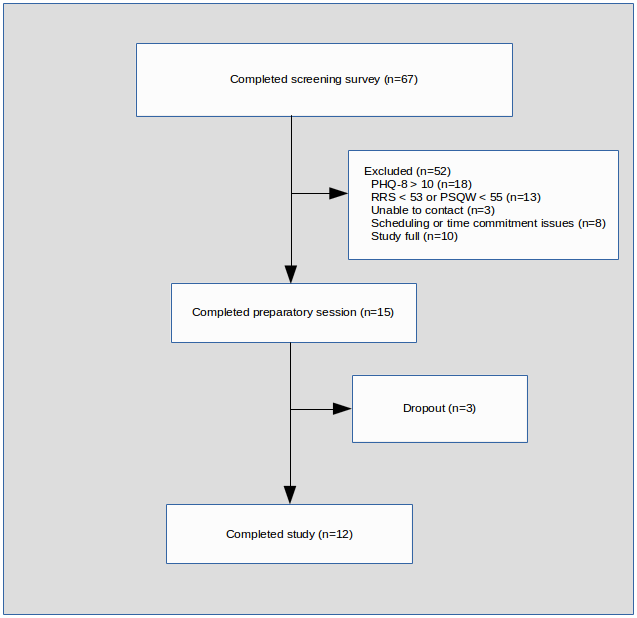
\includegraphics[width=140mm]{/home/paul/Documents/psychology/msc/M210/apprenticeship/dissertation/figure/recruitment.png}
  \caption{Recruitment flowchart}
  \label{flowchart}
\end{figure}

\subsection{Measures and Materials}

All self-report measures were created using Lime Survey
\parencite{limesurvey} and completed online. Ecological validity was
good, with all except the pre self-report measurements taken outside of
a laboratory environment.

\subsubsection{Pre--Post self-report measures}

The following measures were taken before the first and after the last
dot-probe/ABM sessions (\cref{app:surveys}).

\paragraph{RRS}

The Ruminative Responses Scale (RRS) is a 22 item measure
of trait rumination, with items rated 1--4. The
RRS is valid and reliable, having Cronbach's $\alpha$ of .85
\parencite{treynor_rumination_2003}. RRS questions were asked in
relation to the previous 4 weeks, to correspond approximately with the
month before the study (pre) and time within the study (post).

\paragraph{GAD-7}

The GAD-7 is a 7 item measure of Generalised Anxiety Disorder (GAD)
symptoms, with items relating to the previous 2 weeks, and scores rated
0--3. The GAD-7 is an efficient, internally reliable (Cronbach's $\alpha$
> .85) tool for assessing GAD severity in clinical research, with good
test-retest reliability \parencite{spitzerrl_brief_2006}.

\paragraph{PHQ-9}

The 9 item Patient Health Questionnaire Depression (PHQ-9) is a brief,
reliable (Cronbach's $\alpha$ > .85) and valid measure of depression
severity \parencite{kroenke_phq9_2001}. Items are rated 0--3,
and questions relate to the previous 2 weeks.

\paragraph{PSWQ}

The 16 item Penn State Worry Questionnaire (PSWQ) is an internally
consistent measure of trait worry with good test-retest reliability
\parencite{meyer_development_1990}.  Items are rated 1--5.

\subsubsection{Daily measures}

The following measures were taken approximately every 24 hours, except
where sessions were postponed.

\paragraph{GRS}

The Goal Rumination Scale (GRS) is a 7 item measure of state rumination
towards a specific goal \parencite{schultheiss_role_2008}. Items
are rated 1--7, with items 5--7 reversed. Reliability of the GRS is
good (Cronbach's $\alpha$ = .87), based on a single sample of $N$ =
101. Questions on the GRS were asked in relation a ``problem'' rather
than a ``goal'' and in relation to the last 24 hours.

\paragraph{PANAS-SF}

The 10 item, short form Positive and Negative Affect Schedule
\parencite[PANAS-SF,][]{mackinnon_short_1999} measures positive affect
(PA, Cronbach's $\alpha$=.78) and negative affect (NA, Cronbach's
$\alpha$=.87). Items are rated 1--5. Although the PANAS PA
scale has significant negative correlations with depression measures
\parencite{watson_development_1988}, the PANAS-SF PA items (`determined',
`alert', `inspired', `enthusiastic', `excited') do not represent the
negative pole of positive affect. Therefore, to improve detection of our
hypothesised change in depression, we added items `sad' and `depressed'
to the PANAS-SF. Items `anxious' and `worried' were added to assess
our hypothesised changes in anxiety but excluded from analyses due to
their positive correlation with NA\footnote{Of the four items added to
the PANAS-SF, `sad' and `depressed' correlated strongly with each other
weakly with PA items and moderately with the NA scale. Items `anxious'
and `worried' were moderately correlated with NA, but not as highly
as the NA scale itself (\cref{app:mood}). Given these findings and
that PANAS is an established measure, we analysed three mood variables:
positive affect (PA scale), negative affect (NA scale) and depressive
symptoms (`sad' and `depressed' items).}. Questions on the PANAS-SF were
asked in relation to the last 24 hours.

\subsection{Procedure}

\subsubsection{Preparatory session}

Participants met the researcher at the University of Exeter to complete
the initial 1 hour preparatory session. After giving informed, written
consent, they completed baseline measures for RRS, PHQ-9, GAD-7 and
PSWQ online.  Using a procedure based on \textcite{roberts_cueing_2013},
the participant was instructed to select an unresolved current concern
which they rated on a 5 item scale, with items rated 1--9. The concern
was accepted if ratings for the questions \enquote{How much you have
been thinking about it over the last week?} and \enquote{How much does
it bother you now?} were > 5, and the concern was considered unlikely to
resolve within the following 5 weeks. Each participant's preferred concern
met these criteria. Participants wrote a short statement summarising
their concern and recorded the length of time that it had been bothering
them. They then generated their I-words (\cref{app:iwordgen}) and
completed a dot-probe practice block\footnote{Dot-probe practice blocks
used N-word block 7 (\cref{app:nwords} and a set of I-word pairs generated
by the experimenter.}. Participants were given help installing the
computer task, a task information sheet (\cref{app:taskinstructions}) and
a printed calendar for managing their daily sessions, on which they wrote
an implementation intention \parencite{gollwitzer_implementation_1999}
to encourage session completion. The experimenter then prepared the
files required for the computer task and emailed them to the participant.

\subsubsection{Daily sessions}

Participants were instructed to complete all experimental sessions on a
computer at their home. Each day, the experimenter sent participants a
templated email containing instructions on how to complete the session
(\cref{app:reminder}). Participants began each session by completing
the dot-probe task (phase A) or the ABMT, followed by the
dot-probe (phase B). Dot-probe blocks took approximately 5 minutes to
complete and ABMT blocks approximately 15 minutes.

Using Lime Survey, participants uploaded their task data, recorded
whether their concern was still unresolved and complete PANAS-SF and
GRS measures. The experimenter periodically sent additional emails to
motivate participants by notifying them of their progress, to ensure their
well-being if 3 consecutive sessions were skipped, and to prepare them
for the slightly longer task when transitioning to phase B. Participants
provided post-intervention RRS, PHQ-9, GAD-7 and PSWQ measures using
the Lime Survey website within approximately 12 hours of completing
the final session. On exiting the study, all participants were emailed
debrief information (\cref{app:debrief}) and information about sources of
support \cref{app:support} and were paid for their participation.

\subsubsection{Experimental stimuli}

Negative-Neutral (N-word) pairs differed significantly on valence but were
matched for frequency, imageability, familiarity, number of characters
and number of syllables (\cref{app:nwords}). Ideographic word sets
(I-words) were the 6 words rated by participants as most likely to
induce rumination about their chosen current concern, from a maximum
of 10 self-generated words. The experimenter chose I-word pairs by
selecting neutral words matched for frequency, imageability, familiarity,
word length and number of syllables (\cref{app:iwords}). In order
to detect ${generalised}$ changes in attentional bias in relation to
N-word emotional valence, rather than changes in bias to specific N-word
stimuli \parencite{see_reduction_2009}, phase B dot-probe blocks only
contained N-words not previously exposed in any preceding ABM block. An
example randomisation schedule and associated stimulus allocation is
shown in \cref{tab:stim}.


\setlength\tabcolsep{1mm}
\belowrulesep=0pt
\aboverulesep=0pt
\begin{sidewaystable}[!htbp] \centering
\begin{threeparttable}
{\footnotesize
  \begin{tabular}{@{} |l*{19}{|c}|l| @{}}
    \noalign{\hrule height 1.5pt}
    Pre & \multicolumn{2}{c|}{} & \multicolumn{8}{c|}{Phase A} & \multicolumn{9}{c|}{Phase B} & Post \\
    \hline
    RRS & \multicolumn{2}{c|}{} & \multicolumn{6}{c}{} & & ABM\tabfnm{b} N-words: & 1--6 & 1--12 & 1--18 & 1--24 &
    1--30 & 1--36 & 1--42 & 1--48 & 1--54 & RRS \\
    \cmidrule{2-20}
    PSWQ & dot-probe\tabfnm{a} & N-words & 1--6 & 7--12 & 13--18 &
    19--24 & 25--30 & 31--36 & 37--42 & 43--48 & 7--12 & 13--18 & 19--24 & 25-30
    & 31--36 & 37--42 & 43--48 & 49--54 & 55--60 & PSWQ \\
    \cmidrule{3-20}
    PHQ-9 & & I-words & 1--6 & 1--6 & 1--6 & 1--6 & 1--6 & 1--6 & 1--6 & 1--6 & 1--6
    & 1--6 & 1--6 & 1--6 & 1--6 & 1--6 & 1--6 & 1--6 & 1--6 & PHQ-9 \\
    \cmidrule{2-20}
     GAD-7 & & Session & 1 & 2 & 3 & 4 & 5 & 6 & 7 & 8 & 9--11 & 12--14 & 15--18 &
    19--21 & 21--23 & 24--26 & 27--29 & 30--32 & 33--35 & GAD-7 \\
    \hline
    \end{tabular}
} % footnotesize
    \caption{Example randomisation schedule showing stimulus allocation
    and block order where phase A = 8 sessions and phase B = 27 sessions.
    In phase A, dot-probe blocks consisted of 12 word pairs; the 6 I-word
pairs and 6 N-word pairs. Session 1 used pairs 1--6 from the 66 N-word
set, session 2 used pairs 7--12, and so on. Thus, bias associated with
the participant's ideographic words was measured at every session,
whereas the more general negative valence associated with N-words
was distributed across measurement times. In phase B, dot-probe
measurement was preceded by ABM blocks containing only N-words. To guarantee
enough stimuli when randomisation resulted in a long phase B, the same 6
N-words were used for 3 consecutive ABM training sessions. N-words from
previous ABM blocks were included in subsequent ABM blocks. For example,
the first 3 ABM blocks used N-words 1--6 and the subsequent dot-probe
used N-words 7--12. The fourth ABM block used N-words 1--12 and the
subsequent dot-probe used N-words 13--18, and so on. A random draw was
used to select the 192 stimuli for each ABM session. As with phase A,
the 6 I-words were present in every dot-probe block.}
    \label{tab:stim}
\begin{tablenotes}[para,flushleft]
{\footnotesize
  \tabfnt{a}96 trials
  \tabfnt{b}192 trials
}
\end{tablenotes}
\end{threeparttable}
\end{sidewaystable}


\subsubsection{Dot-probe task}

Our version of the dot-probe task\footnote{The dot-probe task was
developed using OpenSesame, an open-source experiment builder for the
social sciences \parencite{mathot_opensesame_2011}. OpenSesame was
chosen as a package which was relatively easy to install on Windows,
Macintosh (OSX ${\geq}$ 10.9) and Linux operating systems, thereby
eliminating any dependencies on a web server for software development
or data collection. Installation instructions for were created
using screen capture software and uploaded to YouTube.} (figure
\ref{fig:dotprobe}) used two sets of visual word-pair stimuli and was
based on \textcite{yang_attention_2015}. Dot-probe blocks consisted
of 96 trials. Each trial began with an 25 x 25 pixel (7 pixel thick)
white fixation cross centred on a black screen. After 500ms, this was
replaced by a word pair from the current stimulus set. One word from the
pair appeared above the fixation cross location and one below. Word pairs
were 125 pixels high with a vertical space between the upper and lower
words such that the stimuli subtended a visual angle of approximately
2$^{\circ}$. Neutral words appeared with equal frequency at the upper
or lower positions. After 1250 ms, the word pair was replaced by either
a greater than (\texttt{>}) symbol or less than (\texttt{<}) symbol at
a random letter location within one of the previous word locations. As
our aim was to guarantee attentional engagement with word stimuli,
this exposure duration was chosen as being slightly higher than the
1000 ms in which vigilance for negative words has been shown to be
positively correlated with measures of depressed mood and vulnerability
\parencite{bradley_attentional_1997}. Furthermore, attentional biases
are more frequently observed when self-relevant negative information is
presented for longer durations \parencite{koster_understanding_2011},
and attentional biases in depression are critically dependent on longer
(1000 ms) exposure durations \parencite{donaldson_rumination_2007}. Probes
appeared with equal frequency at upper and lower locations. Valid keyboard
responses were greater than (\texttt{>}) and less than (\texttt{<}). The
probe remained on the screen until the participant pressed a valid
key. A correct response was recorded if the key-press matched the probe
symbol. There was no feedback for incorrect responses. A blank screen
with a random inter-trial interval (ITI) between 100-500ms followed each
trial. Participants were instructed to respond as quickly and accurately
as possible.

\begin{figure}[!ht]
  \centering
  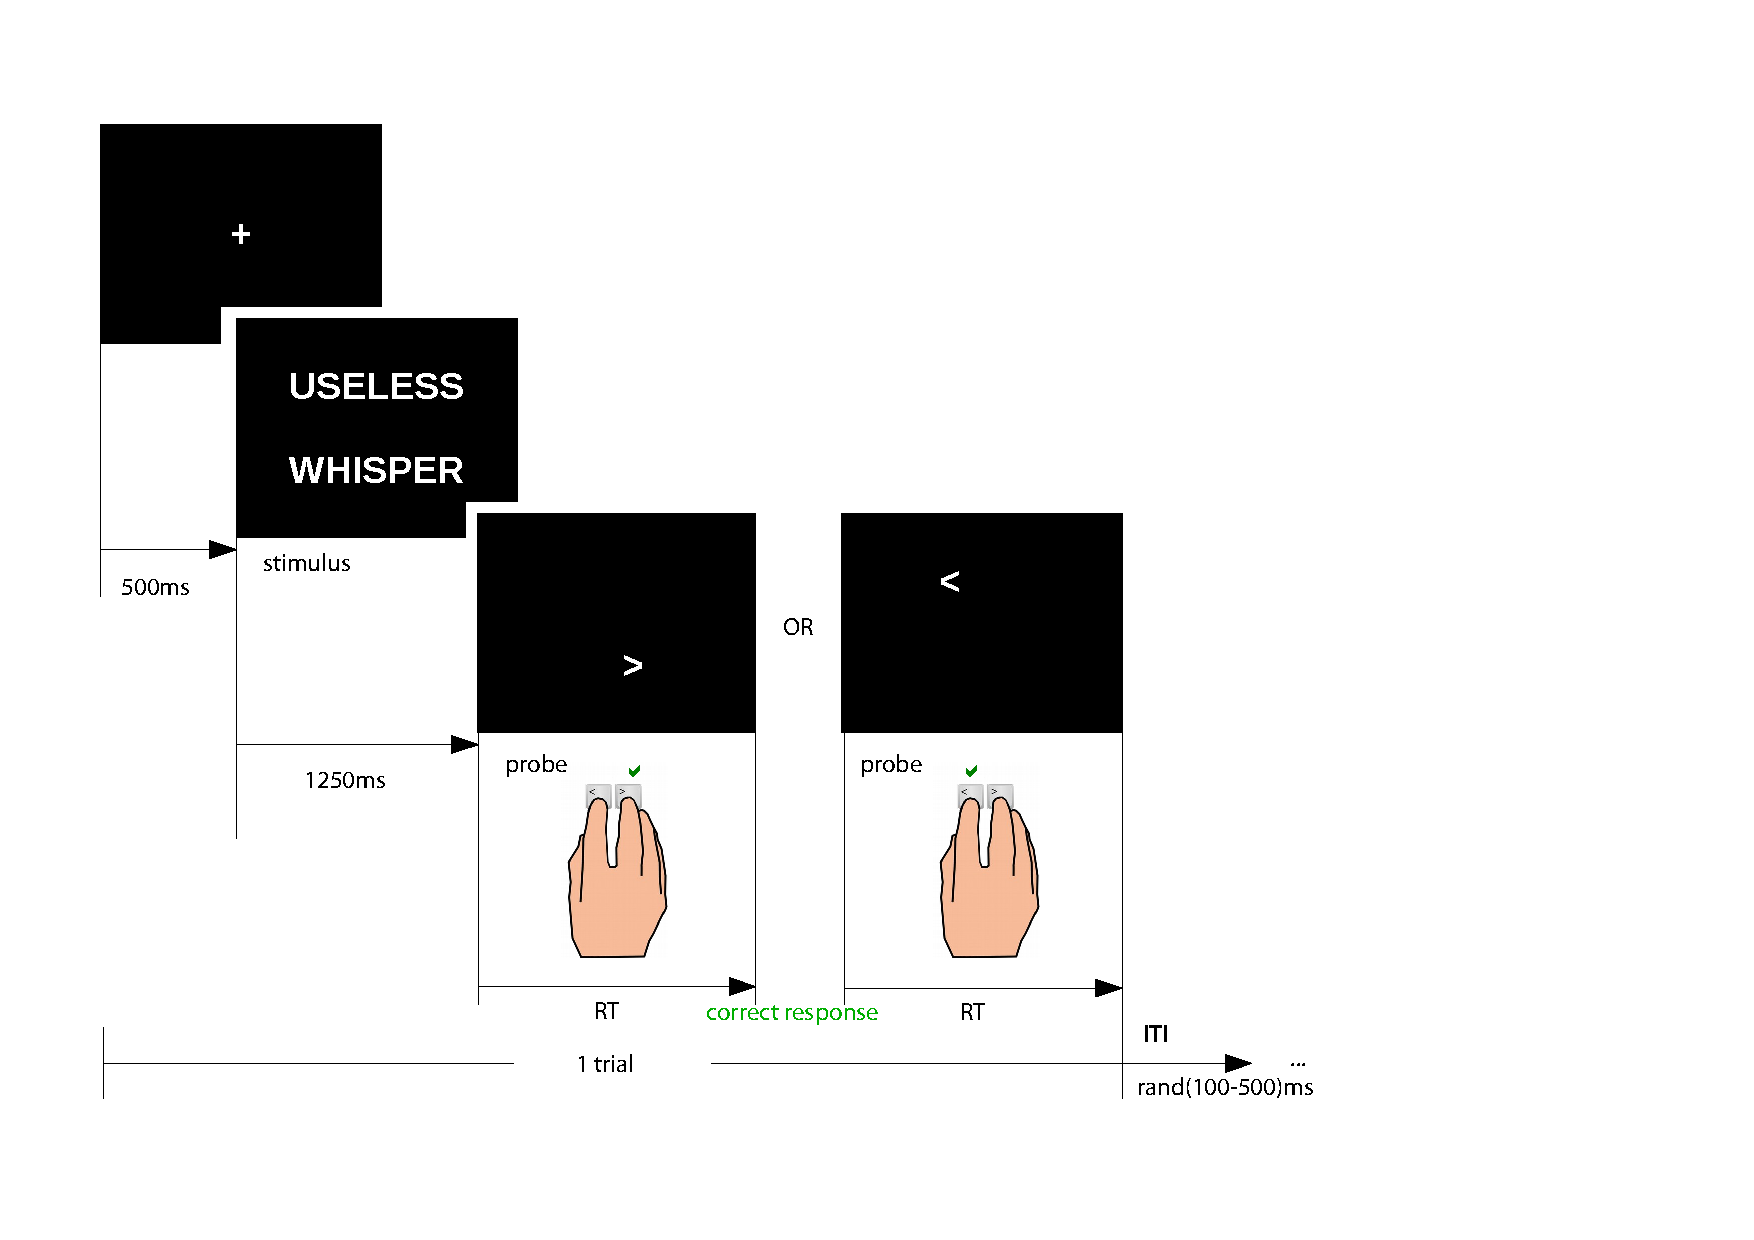
\includegraphics[width=200mm,height=150mm]{/home/paul/Documents/psychology/msc/M210/apprenticeship/dissertation/dot_probe_kb.pdf}
  \caption{Example dot-probe trial for a right-handed participant,
  in which the negative word (\textsf{USELESS}) appears at the upper
  location, and the neutral word (\textsf{WHISPER}) appears at the
  lower location.  Correct responses are shown for a subsequent probe
  appearing at either the upper or lower location.}
  \label{fig:dotprobe}
\end{figure}

\subsubsection{Attentional bias assessment}

After removing inaccurate trials or those with response times (RTs)
exceeding 3 standard deviations beyond the mean, attentional bias scores
were calculated from the remaining RTs using the equation \begin{equation}
  Attentional\ bias\ score = [(NuPl + NlPu) - (NuPu + NlPl)]/2\label{eq:1}
\end{equation} where ${N}$ = Negative word, ${P}$ = Probe, ${u}$ =
upper, ${l}$ = lower \parencite{bradley_attentional_1997}. A bias
towards negative words is reflected in longer latencies for probes
at the opposite location (left-hand side of equation \eqref{eq:1})
and shorter latencies for probes at the same location (right-hand side
of equation \eqref{eq:1}). Therefore, more positive scores reflect an
attentional bias towards (i.e. vigilance for) negative words relative
to neutral words, whereas more negative scores indicate avoidance
\parencite{bradley_attentional_1997}.

\subsubsection{ABMT}

The ABMT task used three minor adjustments to the dot-probe paradigm to
${modify}$, rather than measure attentional bias. First, there were
double the number (192) of trials in each block. Second, only N-word
pairs were used as stimuli. Finally, probes in ABM trials always appeared
at the neutral word location. Thus, correct responses required repeated
orientation of attention away from the negative word in the pair.

% handle weird gaps that appeared between paragraphs near this page
\raggedbottom
\section{Analyses}

Data were analysed using using R version 3.1.0
\parencite{rcoreteam_r_2014}\footnote{Additional R packages used for
analyses were \texttt{corrplot} \parencite{wei_corrplot_2013},
\texttt{lsr} \parencite{navarro_learning_2015},
\texttt{pwr} \parencite{champely_pwr_2015}, \texttt{psy}
\parencite{falissard_psy_2012}, \texttt{SCMA} \parencite{bulte_scma_2015},
\texttt{SCRT} \parencite{bulte_scrt_2015} and \texttt{SCVA}
\parencite{bulte_scva_2015}. Minor modifications were made to the
\texttt{SCVA} package to standardise y-axis ranges and to plot
central tendency, trend and variance lines on the same graph.}.

\subsection{Pre--Post comparisons}

The small ${N}$ meant that pre-post comparisons were underpowered except
for large effects, so our primary analyses were visual inspection
and randomisation tests of daily session measurements. Nevertheless,
two-tailed, paired samples t-tests were used to compare participants'
pre and post ABMT measures of rumination (RRS), depression (PHQ-9),
anxiety (GAD-7) and worry (PSWQ). Whilst these tests were potentially
underpowered, it was noted that the significant post training
effect sizes found by \textcite{yang_attention_2015} were medium
(${d}$=.49) for RRS, large (${d}$=1.50) for depression using BDI-II
\parencite{beck_manual_1996} and large
 (${d}$=.88) for anxiety using STAI-T \parencite{spielberger_manual_1983}.

\subsection{Daily sessions}

Each participant's daily session data was analysed visually and
using randomisation tests comparing phase A and B measures of
attentional bias (I-words and N-words), state rumination (GRS) and
mood (PANAS-SF). Randomisation is a nonparametric approach which
allows inferential statistics to be calculated using data from
a single-case series \parencite{bulte_r_2008}. In an AB design,
the phase sequence (baseline followed by intervention) is fixed,
therefore it is the point at which phase A transitions to phase B
which is randomised. Under the null hypothesis, a test statistic for
a particular set of observations would not differ systematically as a
function of where the transition from A to B occurs. Randomisation tests
hold the observation scores constant and calculate the test statistic
for all possible transition permutations. Once sorted, the ${p}$ value
is the proportion of test statistics greater than or equal to the
observed test statistic \parencite{onghena_customization_2005}. All
randomisation tests were two-tailed (test statistic = \(\lvert
\texttt{A-B}\rvert\)). In addition to the single-case randomisation
tests, a meta-analysis \parencite[][p.64]{onghena_customization_2005}
was carried out across all participants for each outcome
measure\footnote{Meta-analyses were conducted using the R
package \texttt{SCMA} \parencite{bulte_singlecase_2013}.}. With 12
participants, this increases power to detect significance above ${p}$=.05
\parencite[][p.64]{onghena_customization_2005}, even though sensitivity
at the case level was below ${p}$=.05 for participants who completed less
than 35 sessions. The meta-analysis used an additive approach, which
has a greater probability of yielding significant results when there
are treatment effects \parencite{edgington_additive_1972}. Percentage
of nonoverlapping data (PND) was used as a measure of effect
size\footnote{PND was calculated using the R package \texttt{SCMA}, using
\texttt{PND-} for N-words, I-words, NA and depressive symptoms as the
treatment should cause these measures to drop, and \texttt{PND+} for PA
as the treatment should result in an increase in positive affect.}. PND
is frequently used in single-subject research, and is the percentage of
treatment phase observations that do not overlap data in the baseline
phase \parencite{scruggs_pnd_2013}\footnote{\textcite{scruggs_early_1986}
consider treatments with PND scores ${\geq}$ 90\% as highly effective,
scores of 70\%--90\% as fair, scores of 50\%--70\% as questionable
effects, and scores <~ 50\% as unreliable.}. There was no missing data
for daily measures, as all survey questions were mandatory.

\section{Results}

Three participants withdrew from the study; one before completing any
sessions due to concerns that the study would worsen their social anxiety,
another who found the time commitment too great after 5 sessions, and the
third after 24 sessions when a holiday meant that they would be unable
to complete sufficient phase B sessions. Dropout was not predictable for
these participants as their screening scores were not atypical. For the
remaining participants, dot-probe/ABM accuracy was above our ${a priori}$
inclusion threshold of 75\% (\cref{tab:completed}). The current concern
chosen by each participant at the preparatory session remained unresolved
throughout the study.

\belowrulesep=1pt
%\aboverulesep=1pt




\setlength{\tabcolsep}{1pt}
\begin{sidewaystable}
\tiny{
{\sffamily
    \begin{tabular}{@{} crr|r|*{66}{c|} @{}}
        & & \multicolumn{66}{c}{Date} \\[2ex]
\rowcolor{blue!30} \cellcolor{white}
& \cellcolor{white} & \cellcolor{white}
\rot{\shortstack[l]{Sessions\\Completed}} & \cellcolor{white} \rot{\shortstack[l]{Accuracy\\${M}$(${SD}$)}}  & \rot{4/7/2015}  & \rot{5/7/2015}  & \rot{6/7/2015}  & \rot{7/7/2015}  & \rot{8/7/2015}  & \rot{9/7/2015}  & \rot{10/7/2015}  & \rot{11/7/2015}  & \rot{12/7/2015}  & \rot{13/7/2015}  & \rot{14/7/2015}  & \rot{15/7/2015}  & \rot{16/7/2015}  & \rot{17/7/2015}  & \rot{18/7/2015}  & \rot{19/7/2015}  & \rot{20/7/2015}  & \rot{21/7/2015}  & \rot{22/7/2015}  & \rot{23/7/2015}  & \rot{24/7/2015}  & \rot{25/7/2015}  & \rot{26/7/2015}  & \rot{27/7/2015}  & \rot{28/7/2015}  & \rot{29/7/2015}  & \rot{30/7/2015}  & \rot{31/7/2015}  & \rot{1/8/2015}  & \rot{2/8/2015}  & \rot{3/8/2015}  & \rot{4/8/2015}  & \rot{5/8/2015}  & \rot{6/8/2015}  & \rot{7/8/2015}  & \rot{8/8/2015}  & \rot{9/8/2015}  & \rot{10/8/2015}  & \rot{11/8/2015}  & \rot{12/8/2015}  & \rot{13/8/2015}  & \rot{14/8/2015}  & \rot{15/8/2015}  & \rot{16/8/2015}  & \rot{17/8/2015}  & \rot{18/8/2015}  & \rot{19/8/2015}  & \rot{20/8/2015}  & \rot{21/8/2015}  & \rot{22/8/2015}  & \rot{23/8/2015}  & \rot{24/8/2015}  & \rot{25/8/2015}  & \rot{26/8/2015}  & \rot{27/8/2015}  & \rot{28/8/2015}  & \rot{29/8/2015}  & \rot{30/8/2015}  & \rot{31/8/2015}  & \rot{1/9/2015}  & \rot{2/9/2015}  & \rot{3/9/2015}  & \rot{4/9/2015}  & \rot{5/9/2015}  \\[0em]
        \cmidrule{2-68}

 & 5 & 35 & 99\%  & \cellcolor{yellow}1 & \cellcolor{yellow}2 & \cellcolor{yellow}3 & \cellcolor{yellow}4 & \cellcolor{yellow}5 & \cellcolor{yellow}6 & \cellcolor{yellow}7 & \cellcolor{yellow}8 & \cellcolor{yellow}9 & \cellcolor{yellow}10 & \cellcolor{yellow}11 & \cellcolor{yellow}12 & \cellcolor{yellow}13 & \cellcolor{red}X & \cellcolor{yellow}14 & \cellcolor{yellow}15 & \cellcolor{red}X & \cellcolor{yellow}16 & \cellcolor{yellow}17 & \cellcolor{red}X & \cellcolor{red}X & \cellcolor{red}X & \cellcolor{yellow}18 & \cellcolor{yellow}19 & \cellcolor{yellow}20 & \cellcolor{yellow}21 & \cellcolor{yellow}22 & \cellcolor{yellow}23 & \cellcolor{yellow}24 & \cellcolor{yellow}25 & \cellcolor{yellow}26 & \cellcolor{green}27 & \cellcolor{green}28 & \cellcolor{green}29 & \cellcolor{red}X & \cellcolor{green}30 & \cellcolor{green}31 & \cellcolor{green}32 & \cellcolor{green}33 & \cellcolor{green}34 & \cellcolor{green}35 & \cellcolor{white} & \cellcolor{white} & \cellcolor{white} & \cellcolor{white} & \cellcolor{white} & \cellcolor{white} & \cellcolor{white} & \cellcolor{white} & \cellcolor{white} & \cellcolor{white} & \cellcolor{white} & \cellcolor{white} & \cellcolor{white} & \cellcolor{white} & \cellcolor{white} & \cellcolor{white} & \cellcolor{white} & \cellcolor{white} & \cellcolor{white} & \cellcolor{white} & \cellcolor{white} & \cellcolor{white} & \cellcolor{white} \\[0em]
        \cmidrule{2-68}

 & 6 & 25 & 99\%  & \cellcolor{white} & \cellcolor{white} & \cellcolor{white} & \cellcolor{white} & \cellcolor{white} & \cellcolor{white} & \cellcolor{yellow}1 & \cellcolor{yellow}2 & \cellcolor{yellow}3 & \cellcolor{yellow}4 & \cellcolor{yellow}5 & \cellcolor{yellow}6 & \cellcolor{red}X & \cellcolor{yellow}7 & \cellcolor{yellow}8 & \cellcolor{yellow}9 & \cellcolor{yellow}10 & \cellcolor{yellow}11 & \cellcolor{yellow}12 & \cellcolor{yellow}13 & \cellcolor{red}X & \cellcolor{red}X & \cellcolor{red}X & \cellcolor{yellow}14 & \cellcolor{yellow}15 & \cellcolor{yellow}16 & \cellcolor{red}X & \cellcolor{green}17 & \cellcolor{green}18 & \cellcolor{red}X & \cellcolor{red}X & \cellcolor{green}19 & \cellcolor{green}20 & \cellcolor{red}X & \cellcolor{red}X & \cellcolor{red}X & \cellcolor{red}X & \cellcolor{green}21 & \cellcolor{red}X & \cellcolor{red}X & \cellcolor{green}22 & \cellcolor{green}23 & \cellcolor{red}X & \cellcolor{green}24 & \cellcolor{green}25 & \cellcolor{white} & \cellcolor{white} & \cellcolor{white} & \cellcolor{white} & \cellcolor{white} & \cellcolor{white} & \cellcolor{white} & \cellcolor{white} & \cellcolor{white} & \cellcolor{white} & \cellcolor{white} & \cellcolor{white} & \cellcolor{white} & \cellcolor{white} & \cellcolor{white} & \cellcolor{white} & \cellcolor{white} & \cellcolor{white} & \cellcolor{white} \\[0em]
        \cmidrule{2-68}

 & 7 & 35 & 99\%  & \cellcolor{white} & \cellcolor{white} & \cellcolor{white} & \cellcolor{yellow}1 & \cellcolor{yellow}2 & \cellcolor{yellow}3 & \cellcolor{yellow}4 & \cellcolor{yellow}5 & \cellcolor{yellow}6 & \cellcolor{yellow}7 & \cellcolor{yellow}8 & \cellcolor{yellow}9 & \cellcolor{yellow}10 & \cellcolor{yellow}11 & \cellcolor{yellow}12 & \cellcolor{yellow}13 & \cellcolor{yellow}14 & \cellcolor{yellow}15 & \cellcolor{yellow}16 & \cellcolor{yellow}17 & \cellcolor{yellow}18 & \cellcolor{yellow}19 & \cellcolor{yellow}20 & \cellcolor{yellow}21 & \cellcolor{green}22 & \cellcolor{green}23 & \cellcolor{green}24 & \cellcolor{green}25 & \cellcolor{green}26 & \cellcolor{green}27 & \cellcolor{green}28 & \cellcolor{green}29 & \cellcolor{green}30 & \cellcolor{green}31 & \cellcolor{black}{\color{white}X} & \cellcolor{green}33 & \cellcolor{green}34 & \cellcolor{green}35 & \cellcolor{white} & \cellcolor{white} & \cellcolor{white} & \cellcolor{white} & \cellcolor{white} & \cellcolor{white} & \cellcolor{white} & \cellcolor{white} & \cellcolor{white} & \cellcolor{white} & \cellcolor{white} & \cellcolor{white} & \cellcolor{white} & \cellcolor{white} & \cellcolor{white} & \cellcolor{white} & \cellcolor{white} & \cellcolor{white} & \cellcolor{white} & \cellcolor{white} & \cellcolor{white} & \cellcolor{white} & \cellcolor{white} & \cellcolor{white} & \cellcolor{white} & \cellcolor{white} \\[0em]
        \cmidrule{2-68}

 & 8 & 35 & 99\%  & \cellcolor{white} & \cellcolor{white} & \cellcolor{white} & \cellcolor{white} & \cellcolor{white} & \cellcolor{yellow}1 & \cellcolor{yellow}2 & \cellcolor{yellow}3 & \cellcolor{yellow}4 & \cellcolor{yellow}5 & \cellcolor{yellow}6 & \cellcolor{yellow}7 & \cellcolor{yellow}8 & \cellcolor{yellow}9 & \cellcolor{yellow}10 & \cellcolor{yellow}11 & \cellcolor{yellow}12 & \cellcolor{yellow}13 & \cellcolor{yellow}14 & \cellcolor{yellow}15 & \cellcolor{yellow}16 & \cellcolor{yellow}17 & \cellcolor{yellow}18 & \cellcolor{yellow}19 & \cellcolor{yellow}20 & \cellcolor{yellow}21 & \cellcolor{green}22 & \cellcolor{green}23 & \cellcolor{green}24 & \cellcolor{green}25 & \cellcolor{green}26 & \cellcolor{red}X & \cellcolor{red}X & \cellcolor{green}27 & \cellcolor{green}28 & \cellcolor{green}29 & \cellcolor{green}30 & \cellcolor{green}31 & \cellcolor{green}32 & \cellcolor{green}33 & \cellcolor{green}34 & \cellcolor{green}35 & \cellcolor{white} & \cellcolor{white} & \cellcolor{white} & \cellcolor{white} & \cellcolor{white} & \cellcolor{white} & \cellcolor{white} & \cellcolor{white} & \cellcolor{white} & \cellcolor{white} & \cellcolor{white} & \cellcolor{white} & \cellcolor{white} & \cellcolor{white} & \cellcolor{white} & \cellcolor{white} & \cellcolor{white} & \cellcolor{white} & \cellcolor{white} & \cellcolor{white} & \cellcolor{white} & \cellcolor{white} \\[0em]
        \cmidrule{2-68}

 & 9 & 25 & 99\%  & \cellcolor{white} & \cellcolor{white} & \cellcolor{white} & \cellcolor{white} & \cellcolor{white} & \cellcolor{white} & \cellcolor{yellow}1 & \cellcolor{yellow}2 & \cellcolor{yellow}3 & \cellcolor{yellow}4 & \cellcolor{yellow}5 & \cellcolor{yellow}6 & \cellcolor{yellow}7 & \cellcolor{yellow}8 & \cellcolor{green}9 & \cellcolor{green}10 & \cellcolor{green}11 & \cellcolor{red}X & \cellcolor{green}12 & \cellcolor{green}13 & \cellcolor{green}14 & \cellcolor{green}15 & \cellcolor{red}X & \cellcolor{red}X & \cellcolor{green}16 & \cellcolor{green}17 & \cellcolor{red}X & \cellcolor{green}18 & \cellcolor{red}X & \cellcolor{green}19 & \cellcolor{red}X & \cellcolor{green}20 & \cellcolor{red}X & \cellcolor{red}X & \cellcolor{green}21 & \cellcolor{red}X & \cellcolor{red}X & \cellcolor{green}22 & \cellcolor{green}23 & \cellcolor{red}X & \cellcolor{green}24 & \cellcolor{green}25 & \cellcolor{white} & \cellcolor{white} & \cellcolor{white} & \cellcolor{white} & \cellcolor{white} & \cellcolor{white} & \cellcolor{white} & \cellcolor{white} & \cellcolor{white} & \cellcolor{white} & \cellcolor{white} & \cellcolor{white} & \cellcolor{white} & \cellcolor{white} & \cellcolor{white} & \cellcolor{white} & \cellcolor{white} & \cellcolor{white} & \cellcolor{white} & \cellcolor{white} & \cellcolor{white} & \cellcolor{white} \\[0em]
        \cmidrule{2-68}

 & 10 & 35 & 99\%  & \cellcolor{white} & \cellcolor{white} & \cellcolor{white} & \cellcolor{white} & \cellcolor{white} & \cellcolor{yellow}1 & \cellcolor{yellow}2 & \cellcolor{yellow}3 & \cellcolor{yellow}4 & \cellcolor{yellow}5 & \cellcolor{yellow}6 & \cellcolor{yellow}7 & \cellcolor{yellow}8 & \cellcolor{yellow}9 & \cellcolor{red}X & \cellcolor{yellow}10 & \cellcolor{yellow}11 & \cellcolor{yellow}12 & \cellcolor{yellow}13 & \cellcolor{yellow}14 & \cellcolor{red}X & \cellcolor{yellow}15 & \cellcolor{yellow}16 & \cellcolor{red}X & \cellcolor{yellow}17 & \cellcolor{yellow}18 & \cellcolor{yellow}19 & \cellcolor{yellow}20 & \cellcolor{green}21 & \cellcolor{green}22 & \cellcolor{green}23 & \cellcolor{green}24 & \cellcolor{green}25 & \cellcolor{green}26 & \cellcolor{green}27 & \cellcolor{green}28 & \cellcolor{green}29 & \cellcolor{green}30 & \cellcolor{green}31 & \cellcolor{green}32 & \cellcolor{green}33 & \cellcolor{red}X & \cellcolor{red}X & \cellcolor{green}34 & \cellcolor{red}X & \cellcolor{green}35 & \cellcolor{white} & \cellcolor{white} & \cellcolor{white} & \cellcolor{white} & \cellcolor{white} & \cellcolor{white} & \cellcolor{white} & \cellcolor{white} & \cellcolor{white} & \cellcolor{white} & \cellcolor{white} & \cellcolor{white} & \cellcolor{white} & \cellcolor{white} & \cellcolor{white} & \cellcolor{white} & \cellcolor{white} & \cellcolor{white} \\[0em]
        \cmidrule{2-68}

\rot{\rlap{~Participant}} & 11 & 35 & 99\%  & \cellcolor{white} & \cellcolor{white} & \cellcolor{white} & \cellcolor{white} & \cellcolor{white} & \cellcolor{white} & \cellcolor{yellow}1 & \cellcolor{yellow}2 & \cellcolor{yellow}3 & \cellcolor{yellow}4 & \cellcolor{yellow}5 & \cellcolor{yellow}6 & \cellcolor{yellow}7 & \cellcolor{yellow}8 & \cellcolor{red}X & \cellcolor{red}X & \cellcolor{red}X & \cellcolor{red}X & \cellcolor{red}X & \cellcolor{yellow}9 & \cellcolor{yellow}10 & \cellcolor{yellow}11 & \cellcolor{green}12 & \cellcolor{green}13 & \cellcolor{green}14 & \cellcolor{green}15 & \cellcolor{green}16 & \cellcolor{green}17 & \cellcolor{green}18 & \cellcolor{green}19 & \cellcolor{green}20 & \cellcolor{green}21 & \cellcolor{green}22 & \cellcolor{green}23 & \cellcolor{green}24 & \cellcolor{green}25 & \cellcolor{green}26 & \cellcolor{green}27 & \cellcolor{green}28 & \cellcolor{green}29 & \cellcolor{green}30 & \cellcolor{green}31 & \cellcolor{green}32 & \cellcolor{green}33 & \cellcolor{green}34 & \cellcolor{green}35 & \cellcolor{white} & \cellcolor{white} & \cellcolor{white} & \cellcolor{white} & \cellcolor{white} & \cellcolor{white} & \cellcolor{white} & \cellcolor{white} & \cellcolor{white} & \cellcolor{white} & \cellcolor{white} & \cellcolor{white} & \cellcolor{white} & \cellcolor{white} & \cellcolor{white} & \cellcolor{white} & \cellcolor{white} & \cellcolor{white} \\[0em]
        \cmidrule{2-68}

 & 12 & 35 & 99\%  & \cellcolor{white} & \cellcolor{white} & \cellcolor{white} & \cellcolor{white} & \cellcolor{white} & \cellcolor{white} & \cellcolor{white} & \cellcolor{white} & \cellcolor{white} & \cellcolor{white} & \cellcolor{yellow}1 & \cellcolor{yellow}2 & \cellcolor{yellow}3 & \cellcolor{yellow}4 & \cellcolor{yellow}5 & \cellcolor{yellow}6 & \cellcolor{yellow}7 & \cellcolor{yellow}8 & \cellcolor{yellow}9 & \cellcolor{yellow}10 & \cellcolor{yellow}11 & \cellcolor{yellow}12 & \cellcolor{yellow}13 & \cellcolor{yellow}14 & \cellcolor{yellow}15 & \cellcolor{yellow}16 & \cellcolor{green}17 & \cellcolor{green}18 & \cellcolor{green}19 & \cellcolor{green}20 & \cellcolor{green}21 & \cellcolor{green}22 & \cellcolor{green}23 & \cellcolor{green}24 & \cellcolor{green}25 & \cellcolor{green}26 & \cellcolor{green}27 & \cellcolor{green}28 & \cellcolor{green}29 & \cellcolor{green}30 & \cellcolor{red}X & \cellcolor{green}31 & \cellcolor{green}32 & \cellcolor{green}33 & \cellcolor{green}34 & \cellcolor{green}35 & \cellcolor{white} & \cellcolor{white} & \cellcolor{white} & \cellcolor{white} & \cellcolor{white} & \cellcolor{white} & \cellcolor{white} & \cellcolor{white} & \cellcolor{white} & \cellcolor{white} & \cellcolor{white} & \cellcolor{white} & \cellcolor{white} & \cellcolor{white} & \cellcolor{white} & \cellcolor{white} & \cellcolor{white} & \cellcolor{white} \\[0em]
        \cmidrule{2-68}

 & 15 & 27 & 99\%  & \cellcolor{white} & \cellcolor{white} & \cellcolor{white} & \cellcolor{white} & \cellcolor{white} & \cellcolor{white} & \cellcolor{white} & \cellcolor{white} & \cellcolor{white} & \cellcolor{white} & \cellcolor{white} & \cellcolor{white} & \cellcolor{white} & \cellcolor{white} & \cellcolor{yellow}1 & \cellcolor{yellow}2 & \cellcolor{yellow}3 & \cellcolor{yellow}4 & \cellcolor{yellow}5 & \cellcolor{yellow}6 & \cellcolor{yellow}7 & \cellcolor{yellow}8 & \cellcolor{yellow}9 & \cellcolor{yellow}10 & \cellcolor{yellow}11 & \cellcolor{yellow}12 & \cellcolor{yellow}13 & \cellcolor{green}14 & \cellcolor{green}15 & \cellcolor{green}16 & \cellcolor{green}17 & \cellcolor{green}18 & \cellcolor{green}19 & \cellcolor{green}20 & \cellcolor{green}21 & \cellcolor{green}22 & \cellcolor{green}23 & \cellcolor{green}24 & \cellcolor{green}25 & \cellcolor{green}26 & \cellcolor{green}27 & \cellcolor{white} & \cellcolor{white} & \cellcolor{white} & \cellcolor{white} & \cellcolor{white} & \cellcolor{white} & \cellcolor{white} & \cellcolor{white} & \cellcolor{white} & \cellcolor{white} & \cellcolor{white} & \cellcolor{white} & \cellcolor{white} & \cellcolor{white} & \cellcolor{white} & \cellcolor{white} & \cellcolor{white} & \cellcolor{white} & \cellcolor{white} & \cellcolor{white} & \cellcolor{white} & \cellcolor{white} & \cellcolor{white} \\[0em]
        \cmidrule{2-68}

 & 16 & 33 & 99\%  & \cellcolor{white} & \cellcolor{white} & \cellcolor{white} & \cellcolor{white} & \cellcolor{white} & \cellcolor{white} & \cellcolor{white} & \cellcolor{white} & \cellcolor{white} & \cellcolor{white} & \cellcolor{white} & \cellcolor{white} & \cellcolor{white} & \cellcolor{yellow}1 & \cellcolor{yellow}2 & \cellcolor{yellow}3 & \cellcolor{yellow}4 & \cellcolor{yellow}5 & \cellcolor{yellow}6 & \cellcolor{yellow}7 & \cellcolor{yellow}8 & \cellcolor{yellow}9 & \cellcolor{yellow}10 & \cellcolor{red}X & \cellcolor{yellow}11 & \cellcolor{yellow}12 & \cellcolor{yellow}13 & \cellcolor{yellow}14 & \cellcolor{red}X & \cellcolor{red}X & \cellcolor{yellow}15 & \cellcolor{yellow}16 & \cellcolor{green}17 & \cellcolor{green}18 & \cellcolor{red}X & \cellcolor{green}19 & \cellcolor{green}20 & \cellcolor{green}21 & \cellcolor{green}22 & \cellcolor{red}X & \cellcolor{green}23 & \cellcolor{red}X & \cellcolor{red}X & \cellcolor{green}24 & \cellcolor{green}25 & \cellcolor{green}26 & \cellcolor{red}X & \cellcolor{red}X & \cellcolor{green}27 & \cellcolor{green}28 & \cellcolor{green}29 & \cellcolor{red}X & \cellcolor{red}X & \cellcolor{red}X & \cellcolor{red}X & \cellcolor{red}X & \cellcolor{red}X & \cellcolor{red}X & \cellcolor{green}30 & \cellcolor{green}31 & \cellcolor{green}32 & \cellcolor{green}33 & \cellcolor{white} & \cellcolor{white} \\[0em]
        \cmidrule{2-68}

 & 18 & 35 & 99\%  & \cellcolor{white} & \cellcolor{white} & \cellcolor{white} & \cellcolor{white} & \cellcolor{white} & \cellcolor{white} & \cellcolor{white} & \cellcolor{white} & \cellcolor{white} & \cellcolor{white} & \cellcolor{white} & \cellcolor{white} & \cellcolor{white} & \cellcolor{white} & \cellcolor{white} & \cellcolor{white} & \cellcolor{yellow}1 & \cellcolor{yellow}2 & \cellcolor{yellow}3 & \cellcolor{yellow}4 & \cellcolor{yellow}5 & \cellcolor{red}X & \cellcolor{yellow}6 & \cellcolor{yellow}7 & \cellcolor{red}X & \cellcolor{yellow}8 & \cellcolor{red}X & \cellcolor{yellow}9 & \cellcolor{yellow}10 & \cellcolor{yellow}11 & \cellcolor{yellow}12 & \cellcolor{green}13 & \cellcolor{green}14 & \cellcolor{green}15 & \cellcolor{red}X & \cellcolor{green}16 & \cellcolor{red}X & \cellcolor{green}17 & \cellcolor{red}X & \cellcolor{green}18 & \cellcolor{red}X & \cellcolor{green}19 & \cellcolor{red}X & \cellcolor{red}X & \cellcolor{green}20 & \cellcolor{green}21 & \cellcolor{red}X & \cellcolor{green}22 & \cellcolor{green}23 & \cellcolor{red}X & \cellcolor{green}24 & \cellcolor{red}X & \cellcolor{red}X & \cellcolor{green}25 & \cellcolor{green}26 & \cellcolor{green}27 & \cellcolor{green}28 & \cellcolor{green}29 & \cellcolor{green}30 & \cellcolor{green}31 & \cellcolor{green}32 & \cellcolor{green}33 & \cellcolor{green}34 & \cellcolor{green}35 \\[0em]
        \cmidrule{2-68}

 & 19 & 35 & 99\%  & \cellcolor{white} & \cellcolor{white} & \cellcolor{white} & \cellcolor{white} & \cellcolor{white} & \cellcolor{white} & \cellcolor{white} & \cellcolor{white} & \cellcolor{white} & \cellcolor{white} & \cellcolor{white} & \cellcolor{white} & \cellcolor{white} & \cellcolor{white} & \cellcolor{white} & \cellcolor{white} & \cellcolor{white} & \cellcolor{white} & \cellcolor{white} & \cellcolor{white} & \cellcolor{white} & \cellcolor{white} & \cellcolor{white} & \cellcolor{yellow}1 & \cellcolor{yellow}2 & \cellcolor{yellow}3 & \cellcolor{yellow}4 & \cellcolor{yellow}5 & \cellcolor{yellow}6 & \cellcolor{yellow}7 & \cellcolor{yellow}8 & \cellcolor{yellow}9 & \cellcolor{yellow}10 & \cellcolor{yellow}11 & \cellcolor{yellow}12 & \cellcolor{yellow}13 & \cellcolor{yellow}14 & \cellcolor{yellow}15 & \cellcolor{yellow}16 & \cellcolor{yellow}17 & \cellcolor{yellow}18 & \cellcolor{yellow}19 & \cellcolor{yellow}20 & \cellcolor{yellow}21 & \cellcolor{green}22 & \cellcolor{green}23 & \cellcolor{green}24 & \cellcolor{green}25 & \cellcolor{green}26 & \cellcolor{green}27 & \cellcolor{green}28 & \cellcolor{green}29 & \cellcolor{green}30 & \cellcolor{red}X & \cellcolor{red}X & \cellcolor{green}31 & \cellcolor{green}32 & \cellcolor{green}33 & \cellcolor{green}34 & \cellcolor{green}35 & \cellcolor{white} & \cellcolor{white} & \cellcolor{white} & \cellcolor{white} \\[0em]
        \cmidrule{2-68}

    \end{tabular}
    }
  }
    \caption{Participant's session completion patterns}
\end{sidewaystable}




\subsection{Pre--Post Measures}

Comparisons between outcome measures pre and post ABMT are summarised in
\cref{tab:prepost}. There were no outliers (> 3SD) on GAD-7, PHQ-9, PSWQ
or RRS scores before or after ABMT. Cronbach's $\alpha$ was acceptable
for GAD-7 and PSWQ, good for PHQ-9 and and excellent for RRS. There were
no significant pre-post ABMT differences (all ${P}$s {\textgreater} .05)
on any of these outcomes.



\setlength\tabcolsep{1mm}
% latex table generated in R 3.1.0 by xtable 1.7-4 package
% Thu Sep 24 19:08:33 2015
\begin{threeparttable}[ht]
\centering
\caption{Pre--post ABM training comparisons of trait anxiety (GAD-7), depression (PHQ-9), trait worry (PSQW) and trait rumination (RRS).} 
\label{tab:prepost}
{\footnotesize
\begin{tabular}{clrlrrrrcr}
  \toprule 
 & \multicolumn{2}{l}{Pre} & \multicolumn{2}{l}{Post} \\
 \cline{2-5} 
 Measure & ${M}$(${SD}$) & Cronbach's $\alpha$ & ${M}$(${SD}$) & Cronbach's $\alpha$ & ${t}$ & ${df}$ & ${p}$ & CI$_{95\%}$\tabfnm{a}  & Cohen's ${d}$\tabfnm{b}\\
 \midrule 
 GAD-7 & 8.00(3.07) & .75 & 8.67(3.87) & .81 & -1.08 & 11 & .305 & [-2.03, 0.70] & .22 \\ 
  PHQ-9 & 6.83(4.34) & .80 & 6.83(5.70) & .89 & 0.00 & 11 & 1.000 & [-3.32, 3.32] & .00 \\ 
  PSWQ & 47.33(8.16) & .77 & 46.83(9.22) & .81 & 0.34 & 11 & .743 & [-2.77, 3.77] & .06 \\ 
  RRS & 47.67(11.87) & .92 & 45.67(13.72) & .94 & 0.76 & 11 & .462 & [-3.77, 7.77] & .17 \\ 
   \bottomrule 
\end{tabular}
}
\begin{tablenotes}[para,flushleft]
{\footnotesize \tabfnt{a}Confidence interval represents difference in pre and post measures. \tabfnt{b}Cohen's ${d}$ calculated using standard deviation of pre measures.
}
\end{tablenotes}
\end{threeparttable}


\subsection{Visual Analyses}
\label{sec:va}

Visual analyses commonly examine post-treatment changes in central
tendency and linear trends \parencite{morley_graphical_1991}. In the
following graphs, the broadened median (BMED) is used as a measure of
central tendency as it is both sensitive to a reasonable proportion
of the data, and resistant to outliers in relatively small samples
\parencite{morley_graphical_1991}. We expected to see visual differences
in BMED in the hypothesised direction for each outcome\footnote{On
the attentional bias graphs, the change in BMED between phases A
and B is visually small relative to the variability due to outliers
for some participants.}. Plotting linear trends in central tendency
reduces visual bias when estimating trends from raw data points (due to
outliers). The trend lines in following graphs were plotted using the
split middle method \parencite{morley_graphical_1991}\footnote{This
robust method results in two lines where there are an odd number of
points in a phase. Poor alignment between these lines indicates a poor
fit \parencite{morley_graphical_1991}.}. We expected to see changes in
trend in the hypothesised direction for each outcome.

\subsubsection{N-word attentional bias}

Changes in attentional bias for N-word pairs are summarised in
\cref{fig:va-n-a} and \cref{fig:va-n-b}. Our hypothesis predicted
more negative N-word scores in phase B (i.e. increased avoidance).
All participants had an initial BMED score close to 0, indicating a
lack of any large attentional bias in either direction. Relative to
phase A, 7 participants (5, 6, 8, 10, 11, 16 and 19) had more negative
BMED scores, although participant 5 had 2 large, negative scores. In
phase A, linear trends in score increased for 7 participants (5, 6, 8,
11, 15 and notably 12), decreased for 4 participants (9, 16, 18 and 19)
and remained flat for 2 participants (7 and 10). Relative to phase A,
of the phase B trends which were a good fit, participant 11 reversed in
the hypothesised direction, 3 (participants 8, 12 and 15) continued in
the same direction, and 2 (participants 9 and 19) reversed contrary to
the hypothesised direction. In summary, there was no clear support for
our hypothesised decrease in N-word bias score.

\begin{figure}[!htbp]
  \begin{subfigure}[!htbp]{\textwidth}
    \includegraphics[plotwh]{/media/paul/2E95-1293/study/participants/5/p5_n.jpg}
    \includegraphics[plotwh]{/media/paul/2E95-1293/study/participants/6/p6_n.jpg}
    \includegraphics[plotwh]{/media/paul/2E95-1293/study/participants/7/p7_n.jpg}
    \includegraphics[plotwh]{/media/paul/2E95-1293/study/participants/8/p8_n.jpg}
    \includegraphics[plotwh]{/media/paul/2E95-1293/study/participants/9/p9_n.jpg}
    \includegraphics[plotwh]{/media/paul/2E95-1293/study/participants/10/p10_n.jpg}
    \caption{N-word attentional bias scores for participants 5--10.}
    \label{fig:va-n-a}
    \end{subfigure}
\end{figure}

\begin{figure}
\ContinuedFloat
  \begin{subfigure}[!htbp]{\textwidth}
    \includegraphics[plotwh]{/media/paul/2E95-1293/study/participants/11/p11_n.jpg}
    \includegraphics[plotwh]{/media/paul/2E95-1293/study/participants/12/p12_n.jpg}
    \includegraphics[plotwh]{/media/paul/2E95-1293/study/participants/15/p15_n.jpg}
    \includegraphics[plotwh]{/media/paul/2E95-1293/study/participants/16/p16_n.jpg}
    \includegraphics[plotwh]{/media/paul/2E95-1293/study/participants/18/p18_n.jpg}
    \includegraphics[plotwh]{/media/paul/2E95-1293/study/participants/19/p19_n.jpg}
    \caption{N-word attentional bias scores for participants 11, 12, 15, 16, 18 and 19.}
    \label{fig:va-n-b}
  \end{subfigure}
\caption{N-word attentional bias scores. Dashed line = phase transition. \protect\strokeA{} broadened
median, \protect\strokeB{} split middle linear trend.}
\label{fig:va-n}
\end{figure}
\clearpage

\subsubsection{I-word attentional bias}

Changes in attentional bias for I-word pairs are summarised in
\cref{fig:va-i-a} and \cref{fig:va-i-b}. As with N-words, our hypothesis
predicted more negative scores in phase B (i.e. increased avoidance)
and there were no large initial attentional biases in either direction.
Relative to phase A, 9 participants (5, 6, 8, 9, 10, 15, 16, 18 and 19)
had more negative BMED scores. Of the linear trends in phase A which
were a good fit, 6 (participants 7, 8, 10, 18 and 19) increased and 5
(participants 5, 6, 9, 12 and 16) decreased. Of the trends in phase B
which were a good fit, relative to phase A, 2 (participants 18 and 19)
became more negative and 2 (participants 8 and 9) continued in the same
direction. In summary, there was evidence to support our hypothesised
decrease in I-word bias score in BMED, but not the linear trends.

\begin{figure}[!htbp]
  \begin{subfigure}[!htbp]{\textwidth}
    \includegraphics[plotwh]{/media/paul/2E95-1293/study/participants/5/p5_i.jpg}
    \includegraphics[plotwh]{/media/paul/2E95-1293/study/participants/6/p6_i.jpg}
    \includegraphics[plotwh]{/media/paul/2E95-1293/study/participants/7/p7_i.jpg}
    \includegraphics[plotwh]{/media/paul/2E95-1293/study/participants/8/p8_i.jpg}
    \includegraphics[plotwh]{/media/paul/2E95-1293/study/participants/9/p9_i.jpg}
    \includegraphics[plotwh]{/media/paul/2E95-1293/study/participants/10/p10_i.jpg}
    \caption{I-word attentional bias scores for participants 5--10.}
    \label{fig:va-i-a}
  \end{subfigure}
\end{figure}

\begin{figure}
\ContinuedFloat
  \begin{subfigure}[!htbp]{\textwidth}
    \includegraphics[plotwh]{/media/paul/2E95-1293/study/participants/11/p11_i.jpg}
    \includegraphics[plotwh]{/media/paul/2E95-1293/study/participants/12/p12_i.jpg}
    \includegraphics[plotwh]{/media/paul/2E95-1293/study/participants/15/p15_i.jpg}
    \includegraphics[plotwh]{/media/paul/2E95-1293/study/participants/16/p16_i.jpg}
    \includegraphics[plotwh]{/media/paul/2E95-1293/study/participants/18/p18_i.jpg}
    \includegraphics[plotwh]{/media/paul/2E95-1293/study/participants/19/p19_i.jpg}
    \caption{I-word attentional bias scores for participants 11, 12, 15, 16, 18 and 19.}
    \label{fig:va-i-b}
  \end{subfigure}
\caption{I-word attentional bias scores. Dashed line = phase transition. \protect\strokeA{} broadened
median, \protect\strokeB{} split middle linear trend.}
\label{fig:va-i}
\end{figure}
\clearpage

\subsubsection{State rumination (GRS)}

Changes in GRS scores are summarised in \cref{fig:va-grs-a} and
\cref{fig:va-grs-b}. Relative to phase A, 9 participants (5, 6, 8, 9, 10,
11, 15, 18 and 19) had lower phase B BMED GRS scores, indicating our hypothesised
reduction in rumination towards their chosen concern. These reductions
were largest in participants 10, 5 and 11, although initial GRS was
high in participant 11. Phase A GRS showed a downward trend for 10
participants, being especially steep in participants 5, 10, 18 and
19. Participant 12 showed a steep linear increase in phase A. Of the
linear trends in phase B, 7 were a poor fit. The phase A downwards trends
reduced in phase B for participants 8, 11, 18 and 19, becoming slightly
positive for participant 15. In summary, the BMED changes supported our
hypothesised decrease in GRS scores.

\begin{figure}[!htbp]
  \begin{subfigure}[!htbp]{\textwidth}
    \includegraphics[plotwh]{/media/paul/2E95-1293/study/participants/5/p5_grs.jpg}
    \includegraphics[plotwh]{/media/paul/2E95-1293/study/participants/6/p6_grs.jpg}
    \includegraphics[plotwh]{/media/paul/2E95-1293/study/participants/7/p7_grs.jpg}
    \includegraphics[plotwh]{/media/paul/2E95-1293/study/participants/8/p8_grs.jpg}
    \includegraphics[plotwh]{/media/paul/2E95-1293/study/participants/9/p9_grs.jpg}
    \includegraphics[plotwh]{/media/paul/2E95-1293/study/participants/10/p10_grs.jpg}
    \caption{GRS scores (range 1--49) for participants 5--10.}
    \label{fig:va-grs-a}
  \end{subfigure}
\end{figure}

\begin{figure}
\ContinuedFloat
  \begin{subfigure}[!htbp]{\textwidth}
    \includegraphics[plotwh]{/media/paul/2E95-1293/study/participants/11/p11_grs.jpg}
    \includegraphics[plotwh]{/media/paul/2E95-1293/study/participants/12/p12_grs.jpg}
    \includegraphics[plotwh]{/media/paul/2E95-1293/study/participants/15/p15_grs.jpg}
    \includegraphics[plotwh]{/media/paul/2E95-1293/study/participants/16/p16_grs.jpg}
    \includegraphics[plotwh]{/media/paul/2E95-1293/study/participants/18/p18_grs.jpg}
    \includegraphics[plotwh]{/media/paul/2E95-1293/study/participants/19/p19_grs.jpg}
    \caption{GRS scores (range 1--49) for participants 11, 12, 15, 16, 18 and 19.}
    \label{fig:va-grs-b}
  \end{subfigure}
\caption{GRS scores. Dashed line = phase transition. \protect\strokeA{} broadened
median, \protect\strokeB{} split middle linear trend.}
\label{fig:grs}
\end{figure}
\clearpage

\subsubsection{Positive Affect (PA)}

Changes in PA scores are summarised in \cref{fig:va-pa-a} and
\cref{fig:va-pa-b}. We hypothesised that PA would increase in phase
B. Relative to phase A, 7 (participants 5, 9, 10, 11, 15, 18 and notably
6) phase B BMED PA scores increased, 3 participants (8, 12 and 19)
decreased slightly, participant 16 decreased more markedly and participant
7 remained stable. Where there was a linear fit, phase A PA showed an
upward trend for 5 participants (5, 9, 10, 11 and 18) being especially
steep for participant 9, a downward trend for 2 participants (6 and 15)
and was relatively stable for 2 participants (7 and 19). Where there was
a linear fit in both phases, trends continued in the same direction for
participants 11 and 15, and became more negative for participant 19. In
summary, there was no clear support for our hypothesised increase in PA.

\begin{figure}[!htbp]
  \begin{subfigure}[!htbp]{\textwidth}
    \includegraphics[plotwh]{/media/paul/2E95-1293/study/participants/5/p5_pa.jpg}
    \includegraphics[plotwh]{/media/paul/2E95-1293/study/participants/6/p6_pa.jpg}
    \includegraphics[plotwh]{/media/paul/2E95-1293/study/participants/7/p7_pa.jpg}
    \includegraphics[plotwh]{/media/paul/2E95-1293/study/participants/8/p8_pa.jpg}
    \includegraphics[plotwh]{/media/paul/2E95-1293/study/participants/9/p9_pa.jpg}
    \includegraphics[plotwh]{/media/paul/2E95-1293/study/participants/10/p10_pa.jpg}
    \caption{PA scores (range 1--25) for participants 5--10.}
    \label{fig:va-pa-a}
  \end{subfigure}
\end{figure}

\begin{figure}
\ContinuedFloat
  \begin{subfigure}[!htbp]{\textwidth}
    \includegraphics[plotwh]{/media/paul/2E95-1293/study/participants/11/p11_pa.jpg}
    \includegraphics[plotwh]{/media/paul/2E95-1293/study/participants/12/p12_pa.jpg}
    \includegraphics[plotwh]{/media/paul/2E95-1293/study/participants/15/p15_pa.jpg}
    \includegraphics[plotwh]{/media/paul/2E95-1293/study/participants/16/p16_pa.jpg}
    \includegraphics[plotwh]{/media/paul/2E95-1293/study/participants/18/p18_pa.jpg}
    \includegraphics[plotwh]{/media/paul/2E95-1293/study/participants/19/p19_pa.jpg}
    \caption{PA scores (range 1--25) for participants 11, 12, 15, 16, 18 and 19.}
    \label{fig:va-pa-b}
  \end{subfigure}
\caption{PA scores. Dashed line = phase transition. \protect\strokeA{} broadened
median, \protect\strokeB{} split middle linear trend.}
\label{fig:pa}
\end{figure}

\clearpage
\subsubsection{Negative Affect (NA)}

Changes in NA scores are summarised in \cref{fig:va-na-a} and
\cref{fig:va-na-b}. We hypothesised that NA would decrease in phase
B. Relative to phase A, 9 (participants 5, 6, 9, 10, 11, 12, 15, 16 and
18) BMED phase B NA scores decreased. Where there was a linear fit in
phase A, 6 participants (5, 6, 9, 10, 11, 18 and 19) showed an downward
trend (participant 18 being especially steep), participant 15 showed
an upward trend and the trend was relatively flat for participants 12
and 18.  Where there was a linear fit in both phases, trends slowed for
participants 6, continued for participant 11, and reversed sharply from
positive to negative for participant 8. In summary, the BMED changes
supported our hypothesised decrease in NA scores.

\begin{figure}[!htbp]
  \begin{subfigure}[!htbp]{\textwidth}
    \includegraphics[plotwh]{/media/paul/2E95-1293/study/participants/5/p5_na.jpg}
    \includegraphics[plotwh]{/media/paul/2E95-1293/study/participants/6/p6_na.jpg}
    \includegraphics[plotwh]{/media/paul/2E95-1293/study/participants/7/p7_na.jpg}
    \includegraphics[plotwh]{/media/paul/2E95-1293/study/participants/8/p8_na.jpg}
    \includegraphics[plotwh]{/media/paul/2E95-1293/study/participants/9/p9_na.jpg}
    \includegraphics[plotwh]{/media/paul/2E95-1293/study/participants/10/p10_na.jpg}
    \caption{NA scores (range 1--25) for participants 5--10.}
    \label{fig:va-na-a}
  \end{subfigure}
\end{figure}

\begin{figure}
\ContinuedFloat
  \begin{subfigure}[!htbp]{\textwidth}
    \includegraphics[plotwh]{/media/paul/2E95-1293/study/participants/11/p11_na.jpg}
    \includegraphics[plotwh]{/media/paul/2E95-1293/study/participants/12/p12_na.jpg}
    \includegraphics[plotwh]{/media/paul/2E95-1293/study/participants/15/p15_na.jpg}
    \includegraphics[plotwh]{/media/paul/2E95-1293/study/participants/16/p16_na.jpg}
    \includegraphics[plotwh]{/media/paul/2E95-1293/study/participants/18/p18_na.jpg}
    \includegraphics[plotwh]{/media/paul/2E95-1293/study/participants/19/p19_na.jpg}
    \caption{NA scores (range 1--25) for participants 11, 12, 15, 16, 18 and 19.}
    \label{fig:va-na-b}
  \end{subfigure}
\caption{NA scores. Dashed line = phase transition. \protect\strokeA{} broadened
median, \protect\strokeB{} split middle linear trend.}
\label{fig:na}
\end{figure}

\clearpage
\subsubsection{Depression}

Changes in depression\footnote{For brevity, the two-item measure of
${depressive symptoms}$ is henceforth referred to as depression.} scores
are summarised in \cref{fig:va-d-a} and \cref{fig:va-d-b}. Initial
depression scores were moderate to low for all participants. We
hypothesised that depression would decrease in phase B. Relative to phase
A, 7 (participants 6, 8, 9, 11, 12, 15 and 18 ) BMED phase B depression
scores decreased, 4 (participants 5, 10, 16 and 19) increased, and 1
(participant 7) remained the same.  Where there was a linear fit,
phase A NA showed an downward trend for 4 participants (6, 9, 15, 18)
being especially steep for participants 9 and 18, an upward trend for
participant 12 and was relatively flat for 3 participants (5, 7 and
19). Where there was a linear fit in both phases, trends continued
in the same direction for participants 7 and 10, stabilised close to
the bottom of the scale for participants 9, 15 and 18, and increased
sharply for participant 19. In summary, there was no clear support for
our hypothesised decrease in depression score.

\begin{figure}[!htbp]
  \begin{subfigure}[!htbp]{\textwidth}
    \includegraphics[plotwh]{/media/paul/2E95-1293/study/participants/5/p5_d.jpg}
    \includegraphics[plotwh]{/media/paul/2E95-1293/study/participants/6/p6_d.jpg}
    \includegraphics[plotwh]{/media/paul/2E95-1293/study/participants/7/p7_d.jpg}
    \includegraphics[plotwh]{/media/paul/2E95-1293/study/participants/8/p8_d.jpg}
    \includegraphics[plotwh]{/media/paul/2E95-1293/study/participants/9/p9_d.jpg}
    \includegraphics[plotwh]{/media/paul/2E95-1293/study/participants/10/p10_d.jpg}
    \caption{Depression scores (range 1--10) for participants 5--10.}
    \label{fig:va-d-a}
  \end{subfigure}
\end{figure}

\begin{figure}
\ContinuedFloat
  \begin{subfigure}[!htbp]{\textwidth}
    \includegraphics[plotwh]{/media/paul/2E95-1293/study/participants/11/p11_d.jpg}
    \includegraphics[plotwh]{/media/paul/2E95-1293/study/participants/12/p12_d.jpg}
    \includegraphics[plotwh]{/media/paul/2E95-1293/study/participants/15/p15_d.jpg}
    \includegraphics[plotwh]{/media/paul/2E95-1293/study/participants/16/p16_d.jpg}
    \includegraphics[plotwh]{/media/paul/2E95-1293/study/participants/18/p18_d.jpg}
    \includegraphics[plotwh]{/media/paul/2E95-1293/study/participants/19/p19_d.jpg}
    \caption{Depression scores (range 1--10) for participants 11, 12, 15, 16, 18 and 19.}
    \label{fig:va-d-b}
  \end{subfigure}
\caption{Depression scores. Dashed line = phase transition. \protect\strokeA{} broadened
median, \protect\strokeB{} split middle linear trend.}
\label{fig:d}
\end{figure}

\clearpage
\subsection{Inferential Statistics}

\subsubsection{N-word and I-word attentional bias}

N-word and I-word randomisation tests and meta-analysis results are
summarised in \cref{tab:rt}. Although there was a reduction in attentional
bias for I-words for 7 participants (6, 8, 9, 10, 16, 18 and 19), none of
the differences were significant (all ${P}$s < .05). The meta-analysis
across participants was also non-significant (${p}$ = .806). There was
a reduction in attentional bias for N-words in 7 participants (5, 6, 8,
10, 11, 16 and 19), although the difference was only significant (${p}$ =
.05) for participant 11 with an unreliable effect (${PND}$ = 29.17\%). The
meta-analysis across participants was non-significant (${p}$ = .434).

\subsubsection{Rumination (GRS)}

State rumination (GRS) randomisation tests and meta-analysis results
are summarised in \cref{tab:grs}. Although there was a reduction in
GRS score 9 participants (5, 6, 8, 9, 10, 11, 15, 18 and 19), none of
the differences were significant (all ${P}$s < .05). Increases in GRS
for participants 6, 12 and 16 were also non-significant. The
meta-analysis across participants was also non-significant (${p}$ = .563).

\subsubsection{Mood (PA, NA, depression)}

Mood variable (PA, NA and depression) randomisation tests and
meta-analysis are summarised in \cref{tab:panas}. There was a
non-significant increase in PA for 9 participants (5, 6, 7, 9, 10, 11,
12, 15 and 18). Taking our inferential statistics are authoritative,
then contrary to the hypothesised increase in PA, participant 8 showed
a significant decrease (${p}$ = .05). Decreases in PA for participants
16 and 19 were non-significant, as was the meta-analysis across all
participants for PA (${p}$ = .167).  Although there was decrease in
NA for 9 participants (5, 6, 9, 10, 11, 12, 15, 16 and 18), none of
the differences were significant (all ${P}$s < .05). Increases in NA
for participants 7, 8 and 19 were also non-significant, as was the
meta-analysis across all participants for NA (${p}$ = .801). Depression
scores decreased in 5 participants (6, 9, 11, 15 and 18) and increased in
7 participants (5, 7, 8, 10, 12, 16 and 19), however all differences were
non-significant (${P}$s < .05), as was the meta-analysis (${p}$ = .187).

\setlength\tabcolsep{1mm}

% latex table generated in R 3.1.0 by xtable 1.7-4 package
% Thu Sep 24 19:08:28 2015
\begin{sidewaystable}[!htbp]
\begin{threeparttable}
[!htbp]
\centering
\caption{Randomisation tests and meta-analysis for I-word and N-word dot-probe scores\tabfnm{a}. Values in \textbf{bold} indicate reductions in attentional bias after ABM training.} 
\label{tab:rt}
{\footnotesize
\begin{tabular}{ccllrrllrr}
  \toprule 
 & & I words & & & & N words\\
 \cline{3-8} 
 & & A & B & & & A & B\\
 \cline{3-10} 
 Participant & Sessions &
					  ${M}$(${SD}$) & ${M}$(${SD}$) &  ${p}$\tabfnm{b}  & ${PND}$ & ${M}$(${SD}$) &
					  ${M}$(${SD}$) & ~ ${p}$\tabfnm{b}  & ${PND}$\\
 \midrule 
 5 & 35 & -119.35(705.02) & 106.94(1605.23) & .200 & 0.00 & -141.37(713.43) & \textbf{-966.94(1528.88)} & .100 & 22.22 \\ 
  6 & 25 & -137.00(410.27) & \textbf{-275.17(582.41)} & .500 & 11.11 & 26.59(476.47) & \textbf{9.56(238.87)} & .900 & 0.00 \\ 
  7 & 34 & -100.48(284.07) & -54.23(627.51) & .789 & 15.38 & -9.43(344.32) & 19.73(565.87) & .632 & 15.38 \\ 
  8 & 35 & 132.24(434.06) & \textbf{-16.86(479.84)} & .200 & 0.00 & -77.24(340.69) & \textbf{-124.54(799.88)} & .400 & 7.14 \\ 
  9 & 25 & 197.88(313.23) & \textbf{110.56(682.30)} & .600 & 23.53 & -97.75(447.21) & 72.00(749.83) & .400 & 5.88 \\ 
  10 & 35 & 187.45(505.43) & \textbf{-27.03(1503.11)} & .450 & 20.00 & 127.33(334.13) & \textbf{-103.17(987.63)} & .100 & 20.00 \\ 
  11 & 35 & -44.45(455.67) & -26.81(439.53) & .800 & 8.33 & 125.18(316.53) & \textbf{-45.56(398.11)} & .050 & 29.17 \\ 
  12 & 35 & -75.66(818.89) & 97.03(674.28) & .750 & 0.00 & 56.38(743.17) & 254.16(631.97) & .650 & 0.00 \\ 
  15 & 27 & -49.27(415.06) & -22.64(294.00) & .833 & 0.00 & 63.08(363.34) & 93.39(270.90) & 1.000 & 0.00 \\ 
  16 & 35 & -129.56(478.75) & \textbf{-153.39(619.33)} & .750 & 10.53 & -31.44(373.03) & \textbf{-43.08(657.57)} & 1.000 & 10.53 \\ 
  18 & 35 & 53.88(299.62) & \textbf{47.04(311.81)} & .900 & 8.70 & -107.42(209.46) & -22.91(317.86) & .200 & 13.04 \\ 
  19 & 35 & -29.71(411.13) & \textbf{-139.39(289.72)} & .100 & 0.00 & 19.36(283.11) & \textbf{-57.18(161.21)} & .400 & 0.00 \\ 
   \cline{5-5} \cline{9-9}
						
 & & & ${p}$$_{meta}$\tabfnm{c}  &  .806 & & & &  .434 \\
 \bottomrule 
\end{tabular}
}
\begin{tablenotes}[para,flushleft]
{\footnotesize
\tabfnt{a}For both I-words and N-words, more negative scores indicate avoidance, and more positive scores vigilance.
\tabfnt{b}${p}$ value from randomisation test \parencite{bulte_r_2008}
\tabfnt{c}Meta-analytic ${p}$ value \parencite{onghena_customization_2005}.
}
\end{tablenotes}
\end{threeparttable}
\end{sidewaystable}


\input{results/grs.tex}

% latex table generated in R 3.1.0 by xtable 1.7-4 package
% Thu Sep 24 19:08:28 2015
\begin{sidewaystable}[!htbp]
\centering
\caption{Randomisation tests and meta-analysis for positive affect (PA), negative affect (NA) and depression. Values in \textbf{bold} indicate changes in hypothesised direction.} 
\label{tab:panas}
{\scriptsize
\begin{tabular}{ccllrr@{\hspace{2em}}llrr@{\hspace{2em}}llrr}
  \toprule 
 & &  \multicolumn{4}{l}{Positive Affect (PA)\footnote{Cronbach's $\alpha$: median = .83, range = .46--.91}}  &  \multicolumn{4}{l}{Negative Affect (NA)\footnote{Cronbach's $\alpha$: median = .75, range = .25--.95}}  &  \multicolumn{4}{l}{Depression (items 'sad' and 'depressed') \footnote{Cronbach's $\alpha$: median = .83, range = 0.00--.98}} \\
 \cline{3-14} 
 Participant & Sessions & Phase A ${M}$(${SD}$) & Phase B ${M}$(${SD}$)
					  &  ${p}$\footnote{\label{randp1}${p}$ value from randomisation test \parencite{bulte_r_2008}} & ${PND}$ & Phase A ${M}$(${SD}$) & Phase B
					  ${M}$(${SD}$) &  ${p}$\textsuperscript{\ref{randp1}} & ${PND}$ & Phase A ${M}$(${SD}$) &
					  Phase B ${M}$(${SD}$) &  ${p}$\textsuperscript{\ref{randp1}}  & ${PND}$\\
 \midrule 
 5 & 35 & 11.35(4.01) & \textbf{11.67(2.96)} & .750 & 0.00 & 9.92(2.58) & \textbf{8.78(3.35)} & .850 & 0.00 & 5.23(2.41) & 5.44(2.65) & .950 & 0.00 \\ 
  6 & 25 & 9.50(2.34) & \textbf{13.67(3.32)} & .200 & 22.22 & 8.25(2.35) & \textbf{7.11(1.96)} & .400 & 0.00 & 3.19(1.38) & \textbf{2.67(1.32)} & .400 & 0.00 \\ 
  7 & 34 & 14.90(1.89) & \textbf{15.23(2.92)} & .895 & 0.00 & 13.29(1.87) & 14.77(1.64) & .632 & 0.00 & 5.57(0.75) & 5.92(0.28) & .474 & 0.00 \\ 
  8 & 35 & 10.86(3.80) & 9.29(2.20) & .050 & 0.00 & 9.43(2.80) & 10.14(4.04) & .500 & 7.14 & 4.00(1.64) & 4.50(2.65) & .400 & 0.00 \\ 
  9 & 25 & 8.75(3.92) & \textbf{11.06(3.38)} & .100 & 23.53 & 9.12(2.95) & \textbf{8.35(2.74)} & .500 & 0.00 & 3.00(1.41) & \textbf{2.24(0.56)} & .100 & 0.00 \\ 
  10 & 35 & 10.85(2.11) & \textbf{13.93(3.77)} & .400 & 60.00 & 10.50(2.16) & \textbf{8.07(1.53)} & .250 & 6.67 & 2.70(0.80) & 3.33(1.18) & .250 & 0.00 \\ 
  11 & 35 & 8.09(1.64) & \textbf{10.54(3.04)} & .300 & 33.33 & 12.55(1.81) & \textbf{9.75(3.29)} & .750 & 29.17 & 5.36(0.92) & \textbf{4.33(1.13)} & .700 & 20.83 \\ 
  12 & 35 & 12.94(3.80) & \textbf{13.05(4.03)} & 1.000 & 5.26 & 11.88(4.87) & \textbf{10.11(4.99)} & .650 & 0.00 & 4.31(1.92) & 4.53(2.29) & .900 & 0.00 \\ 
  15 & 27 & 7.23(0.93) & \textbf{7.86(2.18)} & .167 & 28.57 & 6.92(1.93) & \textbf{6.14(1.10)} & .333 & 0.00 & 3.92(1.50) & \textbf{3.21(1.12)} & .167 & 0.00 \\ 
  16 & 35 & 10.07(2.55) & 6.53(1.81) & .263 & 0.00 & 10.40(1.18) & \textbf{9.21(2.51)} & .737 & 36.84 & 2.60(0.83) & 3.32(1.34) & .211 & 0.00 \\ 
  18 & 35 & 15.67(1.78) & \textbf{17.04(2.51)} & .800 & 21.74 & 11.42(5.42) & \textbf{8.39(3.97)} & .550 & 0.00 & 4.17(2.86) & \textbf{2.78(1.68)} & .350 & 0.00 \\ 
  19 & 35 & 8.29(1.65) & 6.86(1.23) & .100 & 0.00 & 9.10(2.36) & 9.29(1.14) & .700 & 0.00 & 3.38(0.80) & 3.93(1.14) & .200 & 0.00 \\ 
   \cline{5-5} \cline{9-9} \cline{13-13}
 & & & ${p}$$_{meta}$\footnote{Meta-analytic ${p}$ value \parencite{onghena_customization_2005}.} &  .167 & & & &  .801 & & & &  .187 \\
 \bottomrule 
\end{tabular}
}
\end{sidewaystable}


\clearpage
\section{Discussion}

This study predicted that ABMT would reduce attentional bias, which
would be accompanied by reductions in worry, trait rumination, symptoms
of anxiety and depression, and improvements to mood variables. Contrary
to our hypotheses, we found no reduction in attentional bias towards
towards negative words, no significant differences between pre and post
worry, rumination, symptoms of anxiety and depression. We also found no
overall changes to mood variables in the hypothesised directions. Also
unsupported were our hypotheses that ABMT would reduce rumination towards,
and attentional bias towards words associated with, an ideographic
current concern. These findings do not support the hypothesis that
rumination occurs as a result of an impaired ability to disengage from
negative self-referent information \parencite{koster_understanding_2011}.



We failed to replicate previous findings \parencite{yang_attention_2015}
that ABMT can reduce attentional bias towards sad words, and that
this change is associated with concurrent reductions in trait
rumination and depressive symptoms. One explanation for these null
findings is that the study was underpowered to detect post-ABMT
outcomes. \textcite{yang_attention_2015} found effect sizes of ${d}$=.49
for RRS, ${d}$=1.50 for BDI-II and ${d}$=.88 STAI-T. In the current study,
with 12 participants and $\alpha$ set at .05, two-tailed calculations of
power (1-$\beta$) gave .34 for RRS, 1.00 for BDI-II
and .79 for STAI-T. \textcite{yang_attention_2015} did not
measure worry, but in a similar paradigm, \textcite{enock_attention_2014}
reported ${d}$=.51 for PSWQ which would give the current study
power (1-$\beta$) of .36. Although the study used
different instruments to measure symptoms of depression (PHQ-9
vs. BDI-II) and anxiety (GAD-7 vs. STAI-T), it was not underpowered
in this regard, yet failed to detect effects. In contrast with
\textcite{yang_attention_2015}), participants in this study had low
initial symptoms of depression and anxiety (\cref{tab:prepost}). These
calculations suggest additional power may have been required to detect
changes in rumination (RRS) and worry (PSWQ), both of which showed
moderate but non-significant effects (\cref{tab:prepost}).

As a relatively new psychological task, questions remain regarding
how dot-probe stimulus properties and population characteristics
interact, its reliability as a measure of attentional bias, and
how well ABMT translates into a psychotherapy. Previous research
\parencite{donaldson_rumination_2007,bradley_attentional_1997} strongly
indicates that shorter stimulus presentations are appropriate for
assessing attentional biases associated with anxiety, whereas longer
durations (${\geq}$ 1000 ms) are required when studying depressive
symptoms and rumination. Shorter word presentations in the current
study may have more effectively measured and modified bias, given that
the current sample scored higher on worry than rumination. Stimulus
type (words vs pictures) and sample characteristics (healthy
vs. high symptomatology) are also known to modulate the effects
of ABM on attentional bias, but their interactions remain unclear
\parencite{beard_efficacy_2012}. Important interactions between
stimulus semantics and symptoms have been shown using the Stroop task.
\textcite{mogg_subliminal_1993} found that anxious participants were
slower than depressed and normal participants at naming negative,
but not generally emotional words, and depression-congruent bias
has been shown to depend on self-referent elaborative processing
\parencite{nunn_selective_1997}. The reductions in rumination and
depressive symptoms found by \textcite{yang_attention_2015} were in
participants with mild to severe depressive symptoms, in response to
ABMT using sad and neutral words.  In the current study, the I-words were
highly self-relevant, but the ABMT only included N-word pairs, so it is
possible that words with normative, negative valence were not sufficiently
self-relevant for ABMT to modify bias in this particular sample.

Mixed findings across studies which use the dot-probe could
be also be explained by its poor internal consistency and
test-retest reliability. This has been demonstrated in
clinical and non-clinical samples using both response times
\parencite{schmukle_unreliability_2005} and event-related potentials
\parencite{kappenman_behavioral_2014}. The dot-probe may also be unsuitable for studying attentional biases
and comorbidity. \textcite{musa_selective_2003} found that attentional
bias in patients with social phobia and a concurrent depressive disorder
equivalent to non-patients. Short dot-probe stimulus exposures are
needed to detect biases in anxiety (and possibly worry), whereas longer
exposures are required to detect biases associated with depression and
rumination. The longer exposure used in current study was more likely to
identify identifying ruminative mechanisms rather than those common to
worry and rumination, and this limitation of the dot-probe complicates the
study mixed of anxiety and depression. Finally, although longer stimulus
exposures are likely to result in prolonged processing of self-referent
material, the dot-probe does not necessarily demonstrate attentional
engagement, and as such may be a weak test of the disengagement hypothesis
of depressive rumination \parencite{koster_understanding_2011}.

Directly comparing the current study with previous research on attentional
bias and current concerns is difficult, as this is dominated by studies
which use the Stroop task. However, \parencite{williams_cognitive_1997}
review many studies which suggest that words semantically related
with an individuals schemata surrounding their concerns may be
more influential that the valence of such stimuli. For example,
\parencite{mathews_emotionality_1993} found more Stroop interference in
words judged as highly related to likely concerns or relevant threats,
irrespective of their positive or negative valence. Although dot-probe
studies with anxious patients have failed to find similar evidence
\parencite{musa_selective_2003}, content specificity is consistent
with the mixture of valences in participants I-word ratings (
\cref{app:iwordgen}) in the current study. It is
also suggestive of later, more elaborative information processing common
in depressive rumination.  \textcite[][p. 309]{mogg_subliminal_1993}
have suggested that in the Stroop task, content-specific, elaborative
semantic processing may be more likely with blocked presentation of
stimuli. To test these ideas, the current paradigm could be modified to
use a dot-probe/ABMT with two (or more) words thematically related to
a current concern, paired with thematically neutral words.

Outside of studying current concerns, the goal progress theory of
rumination is very broad and lacking in testable hypotheses. For example,
it is unclear what counts as a ``higher order'' goal, and therefore likely
to trigger rumination \parencite{martin_ruminative_1996}.  Furthermore,
\textcite{martin_ruminative_1996} don't claim that goal discrepancies are
the exclusive cause of rumination. For example, they say the ``rebound
effect'' of thought suppression \parencite{wegner_paradoxical_1987}
can occur in the absence of goal discrepancies, notably in the case
of worry. A related framework with more directly testable hypotheses
\parencite{watkins_habitgoal_2014}, suggests that while goal discrepancies
may cause rumination, this can become a habitual thinking style. Within
this framework, rumination with no overt goal discrepancy may instead
be cued by contingent contexts such as mood, or the physical location
in which it tends to occur. Rumination is especially likely when
contingent responses involve passive focus on abstractly construed,
negative content \parencite{watkins_habitgoal_2014}. The disengagement
hypothesis \parencite{koster_understanding_2011} is especially suited
to, and as yet untested, within this framework. If rumination is a
habitual thinking style, the repetitive nature of ABMT seems promising
as a counter-conditioning technique. The current study used ABMT in a
specific context (at home), but it was not established whether this
context was likely to trigger rumination in each participant. Using
a mobile phone app, it would be relatively easy to test the effects
of ABMT on rumination in contingent contexts. Training attentional
disengagement from negative information is also a central feature of
MBCT \parencite{donaldson_rumination_2007}, suggesting that positive
outcomes may result from encouraging practices such as the ``breathing
space'' \parencite{segal_mindfulnessbased_2012} in rumination-contingent
contexts. These suggestions raise additional questions regarding where,
when and how much ABMT is effective. \textcite{see_reduction_2009} found
signs of reduced attentional avoidance of negative information bias up
to 48 hours post-ABMT, but more research on the longevity of effects
is needed. In the current study, ABMT was relatively ineffective, and
phase B session completion patterns (\cref{tab:completed}) suggest that
people would be unlikely to maintain such intencsive ABMT.

The non-significant effects of ABMT on reducing rumination
in this study support meta-analytic findings that CBM
is relatively ineffective as a treatment for anxiety and
depression. \textcite{hallion_metaanalysis_2011} found that CBM
significantly modified anxiety but not depression, with non-significant
trend toward a larger effects for studies including multiple training
sessions. \textcite{mogoase_clinical_2014} also only found small
therapeutic benefits of ABM for anxiety, although there was less
data for other symptom categories, reflecting a lack of research in
this area. Interpretation biases are likely to be involved in later
information processing stages associated with depressive rumination,
and CBM targeting interpretation (CBM-I) does indeed show larger
effects than ABM \parencite{hallion_metaanalysis_2011}. However,
research in this area is limited and equivocal as to whether
interpretive bias does \parencite{mogg_interpretation_2006} or does not
\parencite{bisson_effect_2007} play a role in depression. Furthermore,
recent studies which demonstrate bias reductions using CBM-I do not
demonstrate symptom change \parencite{micco_efficacy_2014}. Evidence is
also mixed as to whether ABMT could translate into a self-administered
treatment. \textcite{see_reduction_2009} found that Internet delivered
ABMT was effective at inducing avoidance of negative information and
reducing anxiety scores to a subsequent naturalistic stressor. In
the current study, only one participant showed a change in bias
(\cref{tab:rt}) and reduced rumination (\cref{tab:grs}), after 24
ABMT sessions (\cref{tab:stim}). This result is more consistent with
findings that ABMT is effective when delivered in the clinic, but not
when delivered at home \parencite{linetzky_quantitative_2015}.

The inability to demonstrate attentional bias change in this
study is consistent with a general critique of CBM treatments
as having effect sizes too small to be clinically relevant
\parencite{cristea_efficacy_2015}. \textcite{macleod_attentional_2015}
question this finding, arguing that a selection criterion for
meta-analysis should be that studies demonstrate that ABM reduces
both attention bias and symptoms. However, a meta-analysis meeting
this criterion still found effect sizes small for anxiety and
non-significant for depression \textcite{mogoase_clinical_2014}.
\textcite{cuijpers_psychotherapies_2015} conclusion is that research
seeking new psychotherapies for depression is misguided, given the many
existing therapies and the difficulty demonstrating relative efficacy
with sufficient statistical power. Thus, the imminent emergence
of cheap, computer-based therapies for treating anxiety and depression
seems unlikely. One way to address the gap between demand and supply
for treating emotional disorders is to focus research on cheaper ways,
such as I-CBT, of delivering existing psychological therapies known to
be effective. However, cognitive biases clearly play a role in emotional
disorders. Future research in this area may explain why bias modification
is relatively ineffective and may also contribute to explaining why
existing treatments are only partially effective.

This study had a number of limitations. First, it lacked
a control condition. Multiple baseline case-series designs
provide some controls against alternative explanations of
effects including regression to the mean, baseline assessment
effects, extraneous events correlated with phase transition
\parencite{watson_nonconcurrent_1981,watkins_ruminationfocused_2007}.
However, as an exploratory study, limiting Type I error rates was not
a priority and a control condition could be added to a subsequent study
there been significant findings. The study would have benefited from a
more reliable state measure of depressive symptoms than the ad-hoc two
item scale used. Similarly, the validity of the GRS could be questioned,
especially as the the scale valence was modified to refer to a ``problem''
rather than a ``goal''. For consistency with previous research
\parencite{see_reduction_2009}, outcome variables should be measured
post ABMT in response to a naturalistic stressor.

To conclude, the null findings in this study are in line with other
mixed findings in the attentional bias measurement and modification
literature. However, the field has no shortage of theory or hypotheses,
but existing tasks have a limited ability to validate them. Future work
should look for approaches which improve on the Stroop and dot-probe
tasks as measures and modifiers of attentional bias. In the short term,
I-CBT may be the best means of reducing treatment costs. Future work
should test the disengagement hypothesis and possibly MBCT within the
habit-goal framework. Randomisation tests were shown to be complementary
to visual analyses of case-series data.

\printbibliography

%% CAVEAT: \appendices environment breaks \cleveref
\newpage
\appendix
\appendixpage

\setcounter{tocdepth}{1}
\startcontents[sections]
\printcontents[sections]{l}{1}
%\addappheadtotoc
%\todo{appendices: 4000 words max (~250 words/page i.e. 16 pages)}

\section{Survey Measures}
\label{app:surveys}

\begin{sidewaysfigure}[hp]
\includegraphics[width=270mm]{figure/rrs.png}
\caption{Ruminative Responses Scale (RRS) administered using Lime Survey}
\end{sidewaysfigure}

\begin{sidewaysfigure}[hp]
\includegraphics[width=250mm]{figure/gad7.png}
\caption{GAD-7 administered using Lime Survey}
\end{sidewaysfigure}

\begin{sidewaysfigure}[hp]
\includegraphics[width=250mm]{figure/phq9.png}
\caption{PHQ-9 administered using Lime Survey}
\end{sidewaysfigure}

\begin{sidewaysfigure}[hp]
\includegraphics[width=250mm]{figure/pswq.png}
\caption{Penn State Worry Questionnaire (PSWQ) administered using Lime Survey}
\end{sidewaysfigure}

\begin{sidewaysfigure}[hp]
\includegraphics[width=250mm]{figure/panas.png}
\caption{Positive and Negative Affect Schedule (PANAS-SF) administered using Lime Survey}
\end{sidewaysfigure}

\begin{sidewaysfigure}[hp]
\includegraphics[width=250mm]{figure/grs.png}
\caption{Goal Rumination Scale (GRS) administered using Lime Survey}
\end{sidewaysfigure}

\section{Correlations for PANAS-SF and additional mood items}
\label{app:mood}

\begin{figure}[!htbp]
\caption{Correlations PANAS-SF and additional items `sad',`depressed',`anxious',`worried'.}
\centering
  \begin{subfigure}[!htbp]{\textwidth}
    \includegraphics[width=110mm,height=110mm]{figure/PAvs_sad_depressed.jpg}
    \caption{Correlations between PA items, `sad' and `depressed'}
  \end{subfigure}
  \begin{subfigure}[!htbp]{\textwidth}
    \includegraphics[width=110mm,height=110mm]{figure/NAvs_sad_depressed.jpg}
    \caption{Correlations between NA items, `sad' and `depressed'}
  \end{subfigure}
\end{figure}

\begin{figure}
\ContinuedFloat
\centering
  \begin{subfigure}[!htbp]{\textwidth}
    \includegraphics[width=110mm,height=110mm]{figure/NAvs_anxious_worried.jpg}
    \caption{Correlations between NA items, `anxious' and `worried'}
  \end{subfigure}
\end{figure}

\section{N-word stimulus pairs}
\label{app:nwords}

The Sussex Affective Word List (SAWL) \parencite{citron_how_2014} was
used to create 66 N-word stimulus pairs. Starting with 66 words rated
most negative and most neutral, pairs were created by matching words
of equivalent character length, drawing additional words from the SAWL
as necessary to ensure that all pairs were matched on length. A small
number of pairs which appeared to be semantically related were adjusted
by replacing the neutral word in the pair with an alternative from
the SAWL. Independent samples t-tests showed significant differences
(${P}$s {\textless} .001) for mean ratings of valence and arousal
(\cref{tab:nwordcharacteristics}). Pairs were matched for frequency,
imageability, familiarity, number of characters and number of syllables
(all ${P}$s {\textgreater} .16) (\cref{tab:nwordcharacteristics}). In
addition, the mean valence between members of any pair was at least 1.44
(Mean: 2.15, ${SD}$ = 0.37). To form the stimulus blocks, pairs were
ranked by descending mean valence difference.  The 6 pairs with the lowest
difference were assigned to the ``spare'' block, used where I-words were
present in the N-word set. The remaining 60 pairs were divided at every
10 word boundary, forming 6 groups. Each experimental block of 6 words
was created by taking the top pair from each group, until all groups
were exhausted, thereby creating 10 blocks with a mixture of valence
differences. The complete N-word list can be seen in \cref{tab:nwordlist}.

\begin{sidewaystable}[!htbp]
\caption{N-word stimulus pairs used in dot-probe and ABMT}
\label{tab:nwordlist}
{\tiny
  \begin{tabular}{cllllll}\hline%
    Block & Pair 1 & Pair 2 & Pair 3 & Pair 4 & Pair 5 & Pair 6\\\hline 
    \csvreader[late after line=\\]{../experiment/66_nwords.csv}{Block=\block}%
      {\block & \textsf{\csvcolii}-\textsf{\csvcoliii} & \textsf{\csvcoliv}-\textsf{\csvcolv} &
      \textsf{\csvcolvi}-\textsf{\csvcolvii} & \textsf{\csvcolviii}-\textsf{\csvcolix} &
      \textsf{\csvcolx}-\textsf{\csvcolxi} & \textsf{\csvcolxii}-\textsf{\csvcolxiii}}%
    \hline
  \end{tabular}
}
\end{sidewaystable}

% latex table generated in R 3.1.0 by xtable 1.7-4 package
% Thu Sep 24 19:08:33 2015
\begin{table}[ht]
\centering
\caption{Dimensional characteristics of Negative-Neutral word pairs} 
\label{tab:nwordcharacteristics}
{\footnotesize
\begin{tabular}{lrrrrrrr}
  \toprule 
 &  \multicolumn{2}{l}{Negative words}  &  \multicolumn{2}{l}{Neutral words} \\
 &  \multicolumn{2}{c}{(${N}$ = 66)}  &  \multicolumn{2}{c}{(${N}$ = 66)} \\
 \cline{2-5} 
 Dimension & Mean & ${SD}$ & Mean & ${SD}$ & ${t}$ & ${p}$ & CI$_{95\%}$\\
 \midrule 
 valence & -1.78 & 0.38 & 0.29 & 0.36 & -32.26 & $<$ .001 & [-2.20, -1.94] \\ 
  arousal & 4.60 & 0.67 & 2.44 & 0.56 & 20.10 & $<$ .001 & [1.94, 2.37] \\ 
  imageability & 4.05 & 1.13 & 3.99 & 1.50 & 0.27 & .785 & [-0.39, 0.52] \\ 
  familiarity & 4.50 & 0.71 & 4.49 & 1.01 & 0.08 & .933 & [-0.29, 0.31] \\ 
  frequency & 36.77 & 39.11 & 48.91 & 56.69 & -1.43 & .155 & [-28.91, 4.63] \\ 
  syllables & 1.92 & 0.66 & 2.05 & 0.90 & -0.88 & .381 & [-0.39, 0.15] \\ 
  characters & 6.39 & 1.99 & 6.39 & 1.99 & 0.00 & 1.000 & [-0.69, 0.69] \\ 
   \bottomrule 
\end{tabular}
}
\end{table}


\section{I-word stimulus pairs}
\label{app:iwords}

Due to the unpredictability of I-words, and the limited number of words
in the SAWL \parencite{citron_how_2014}, a larger data set was required
to matched pairs to I-words. A database of neutrally valenced words was
created including frequency, imageability, familiarity, word length and
number of syllables attributes from the MRC psycholinguistic database
\parencite{wilson_mrc_1988}. A separate table was added to the database
containing 1030 word valence means from the Affective Norms for English
Words (ANEW) dataset \parencite{bradley_affective_1999}.

Two different matching approaches were used, depending on whether each
I-word word was present in, or absent from, the MRC database.  If present,
a neutral pair was selected from a pool of words having a frequency
{\textpm}15\% that of the I-word, an ANEW valence mean (range 1-9)
between 4.00 and 6.00 and an equal number of characters.  After selecting
a pool of matched words on the preceding criteria, a best match was
found by inspection of candidate words based on number of syllables,
imageability and familiarity.  Some I-words, such as long words or high
frequency words, could not be matched using these criteria due to lack of
available data. In these cases, a word with the most neutral valence was
chosen that also minimised differences in length and frequency between
the word pair. I-words absent from the MRC database (including proper
nouns) were paired with words selected from a pool of 56 words having a
frequency of 1 (on the assumption that words missing from the database
would most likely be of low frequency), and for which an ANEW valence
rating was available.  A word was selected from this pool having an ANEW
valence mean between 4.00 and 6.00 and an equal number of characters
to the I-word. If an I-word or its pair was a member of the N-word set,
that N-word pair was substituted with the next available pair from the
spare N-words block with the largest difference in valence. Resulting
I-word pairs were validated by the experimenter's supervisor. The final
sets of I-word pairs for each participant are shown in \cref{tab:iwords}
and their characteristics in \cref{tab:iwordcharacteristics}.

\label{app:iwordlist}
% latex table generated in R 3.1.0 by xtable 1.7-4 package
% Thu Sep 24 19:08:34 2015
\begin{sidewaystable}[!ph]
\begin{threeparttable}
[ht]
\centering
\caption{Words chosen by each participant as likely to initiate rumination over their current concern (I-words) and matched pairs selected by the experimenter (\textsf{WORD}---\textsf{PAIR}).} 
\label{tab:iwords}
{\tiny
\begin{tabular}{clcccccc}
  \toprule 
 Participant & Concern duration\tabfnm{1} & Pair 1 & Pair 2 & Pair 3 & Pair 4 & Pair 5 & Pair 6\\
\midrule 
 5 & 1 month 3 days & \textsf{SETTLE}---\textsf{BARREL} & \textsf{MARRIAGE}---\textsf{HOSPITAL} & \textsf{AUSTRALIA}\tabfnm{a}{---}\textsf{EMBATTLED} & \textsf{JOB}---\textsf{AIR} & \textsf{LONELY}---\textsf{BUTTER} & \textsf{FAMILY}---\textsf{HISTORY} \\ 
  6 & 2 years & \textsf{DANCE}---\textsf{GLASS} & \textsf{TECHNIQUE}---\textsf{ORCHESTRA} & \textsf{DEPENDENT}---\textsf{INNOCENT} & \textsf{INFERIOR}---\textsf{UMBRELLA} & \textsf{FRUSTRATE}---\textsf{APPLIANCE} & \textsf{UNABLE}---\textsf{AVENUE} \\ 
  7 & 1 year & \textsf{TRAINING}---\textsf{BUILDING} & \textsf{STRUCTURE}---\textsf{ORCHESTRA} & \textsf{FRUSTRATE}---\textsf{APPLIANCE} & \textsf{SUCCESS}---\textsf{MACHINE} & \textsf{TALK}---\textsf{FALL} & \textsf{SLICK}---\textsf{TRUNK} \\ 
  8 & 8 years & \textsf{FAMILY}---\textsf{OFFICE} & \textsf{MATURE}---\textsf{PENCIL} & \textsf{VISIT}---\textsf{GLASS} & \textsf{CAR}---\textsf{AIR} & \textsf{TIME}---\textsf{PART} & \textsf{BUSY}---\textsf{ITEM} \\ 
  9 & 6 months & \textsf{THESIS}---\textsf{LOCKER} & \textsf{COMPLETE}---\textsf{BUILDING} & \textsf{OVERWHELM}---\textsf{AVALANCHE} & \textsf{STRESS}---\textsf{CORNER} & \textsf{TIME}---\textsf{PART} & \textsf{PROGRESS}---\textsf{HOSPITAL} \\ 
  10 & 3 months & \textsf{STRESS}---\textsf{CORNER} & \textsf{FAILING}---\textsf{CABINET} & \textsf{FFFFFFF}\tabfnm{a}{---}\textsf{GLACIER} & \textsf{TELEPHONE}---\textsf{ORCHESTRA} & \textsf{MMMMMM}\tabfnm{a}{---}\textsf{TAMPER} & \textsf{TIME}---\textsf{PART} \\ 
  11 & 2 months & \textsf{STUPID}---\textsf{BARREL} & \textsf{SCIENCE}---\textsf{SERIOUS} & \textsf{TARGET}---\textsf{ENGINE} & \textsf{FFFFFFF}\tabfnm{a}{---}\textsf{KETCHUP} & \textsf{FAILURE}---\textsf{PATIENT} & \textsf{LOSING}---\textsf{CELLAR} \\ 
  12 & 1 year 1 month & \textsf{STUDENT}---\textsf{SERIOUS} & \textsf{SOCIAL}---\textsf{OFFICE} & \textsf{AGE}---\textsf{AIR} & \textsf{KENT}\tabfnm{a}{---}\textsf{FROG} & \textsf{DUTY}---\textsf{ITEM} & \textsf{FRIENDSHIP}---\textsf{RESTAURANT} \\ 
  15 & 1 year 6 months & \textsf{FRUSTRATE}---\textsf{APPLIANCE} & \textsf{ANGER}---\textsf{WAGON} & \textsf{FAILURE}---\textsf{PATIENT} & \textsf{TIRING}---\textsf{KETTLE} & \textsf{CONFLICT}---\textsf{RESERVED} & \textsf{GUILT}---\textsf{PAINT} \\ 
  16 & 21 years & \textsf{FEAR}---\textsf{FARM} & \textsf{PANIC}---\textsf{HABIT} & \textsf{DREAD}---\textsf{TRUNK} & \textsf{PRESSURE}---\textsf{BUILDING} & \textsf{POINTLESS}---\textsf{REPENTANT} & \textsf{FRAUD}---\textsf{SALAD} \\ 
  18 & 8 months 19 days & \textsf{THESIS}---\textsf{LOCKER} & \textsf{CAREER}---\textsf{DETAIL} & \textsf{FINISHING}---\textsf{LIGHTNING} & \textsf{WRITING}---\textsf{MACHINE} & \textsf{FAILURE}---\textsf{PATIENT} & \textsf{DEPRESSION}---\textsf{RESTAURANT} \\ 
  19 & 2 months 25 days & \textsf{INDECISIVE}---\textsf{SKYSCRAPER} & \textsf{TEIGNMOUTH}\tabfnm{a}{---}\textsf{NONCHALANT} & \textsf{FARM}---\textsf{ARMY} & \textsf{SMOKE}---\textsf{BENCH} & \textsf{SURF}---\textsf{FROG} & \textsf{REJECTION}---\textsf{APPLIANCE} \\ 
   \bottomrule 
\end{tabular}
}
\begin{tablenotes}[para,flushleft]
{\footnotesize \tabfnt{1}Answer to the question \enquote{How long has this been a difficulty for you?} at the start of the study. \tabfnt{2}Female and male names redacted with equivalent number of \textsf{F} or \textsf{M} characters respectively. \tabfnt{a}I-word not in database.}
\end{tablenotes}
\end{threeparttable}
\end{sidewaystable}
% latex table generated in R 3.1.0 by xtable 1.7-4 package
% Thu Sep 24 19:08:34 2015
\begin{sidewaystable}[!ph]
\begin{threeparttable}
[ht]
\centering
\caption{Characteristics of each participant's I-words and matched pairs.} 
\label{tab:iwordcharacteristics}
{\footnotesize
\begin{tabular}{cllllllll}
  \toprule 
 & \multicolumn{4}{l}{I-words ${M}$(${SD}$)} & \multicolumn{4}{l}{Pairs ${M}$(${SD}$)}\\
 \cline{2-9} 
 Participant & Frequency\tabfnm{1} & Imageability\tabfnm{2} & Familiarity\tabfnm{2} & Valence\tabfnm{3} & Frequency\tabfnm{1} & Imageability\tabfnm{2} & Familiarity\tabfnm{2} & Valence\tabfnm{4} \\
\midrule 
 5 & 120.50(135.10)\tabfnm{a} & 387.50(300.55)\tabfnm{b} & 341.00(268.90)\tabfnm{b} & -0.50(2.17) & 117.50(125.23) & 470.33(235.02)\tabfnm{c} & 443.67(234.05)\tabfnm{c} & 5.23(0.64) \\ 
  6 & 42.50(33.00) & 271.00(296.95)\tabfnm{c} & 211.67(236.68)\tabfnm{c} & -1.17(1.72) & 40.17(35.93) & 524.67(48.19) & 546.50(91.78) & 5.42(0.51) \\ 
  7 & 84.17(67.15) & 285.00(313.33)\tabfnm{c} & 212.83(234.45)\tabfnm{c} & -1.00(0.89) & 80.50(67.27) & 539.83(46.64) & 567.00(31.31) & 5.11(0.62) \\ 
  8 & 400.33(599.34) & 486.67(244.86)\tabfnm{c} & 410.00(222.89)\tabfnm{c} & -1.83(0.75) & 199.83(176.27) & 584.50(25.96) & 478.17(110.81) & 5.32(0.53) \\ 
  9 & 336.33(622.38) & 201.50(312.16)\tabfnm{c} & 125.67(196.01)\tabfnm{c} & -1.67(2.07) & 149.17(183.03) & 537.83(72.37) & 540.17(99.52) & 4.71(0.77) \\ 
  10 & 300.17(637.76)\tabfnm{a} & 286.67(315.88)\tabfnm{b} & 247.83(285.18)\tabfnm{b} & -2.67(0.82) & 115.67(193.31) & 424.83(217.09)\tabfnm{c} & 436.50(234.81)\tabfnm{c} & 5.02(0.71) \\ 
  11 & 53.00(48.20)\tabfnm{a} & 278.17(304.94)\tabfnm{b} & 206.83(227.32)\tabfnm{b} & -0.83(2.14) & 50.50(43.14) & 358.50(237.43)\tabfnm{c} & 481.33(237.42) & 5.09(0.43) \\ 
  12 & 137.83(143.91)\tabfnm{a} & 470.17(234.59)\tabfnm{b} & 389.67(212.85)\tabfnm{b} & -0.33(2.66) & 120.67(111.14) & 568.67(37.69) & 490.17(110.26) & 5.73(0.68) \\ 
  15 & 38.33(32.35) & 444.17(218.68)\tabfnm{c} & 353.17(177.59)\tabfnm{c} & -3.00(0.00) & 35.50(31.60) & 429.33(214.47)\tabfnm{c} & 373.50(290.14)\tabfnm{c} & 5.25(0.25) \\ 
  16 & 58.67(77.89) & 427.67(215.33)\tabfnm{c} & 350.00(177.88)\tabfnm{c} & -2.83(0.41) & 54.33(69.55) & 465.50(231.70)\tabfnm{c} & 451.33(231.59)\tabfnm{c} & 5.21(0.59) \\ 
  18 & 52.67(45.20) & 383.67(299.02)\tabfnm{c} & 308.00(242.21)\tabfnm{c} & -1.67(1.51) & 54.17(38.84) & 447.17(222.90)\tabfnm{c} & 480.00(236.97)\tabfnm{c} & 4.89(0.63) \\ 
  19 & 30.17(48.93)\tabfnm{a} & 351.00(276.64)\tabfnm{b}\tabfnm{c} & 347.17(288.03)\tabfnm{b}\tabfnm{c} & -0.67(2.58) & 29.33(51.99) & 482.00(64.88) & 541.17(88.80) & 5.13(0.55) \\ 
   \bottomrule 
\end{tabular}
}
\begin{tablenotes}[para,flushleft]
{\footnotesize \tabfnt{1}Frequency norms from \textcite{kucera_computational_1967}. \tabfnt{2}Merged from three sets of norms \parencite{wilson_mrc_1988}. \tabfnt{3}Participant's subjective valence rating using procedure from \textcite{citron_how_2014}. \tabfnt{4} Valence norms from \textcite{bradley_affective_1999} \tabfnt{a}Frequency of 1 assumed for I-words not in database.\tabfnt{b}Missing values were set to 0 for I-words not in database.
\tabfnt{c}Includes one or more 0 values likely to be missing data rather than normative values.}
\end{tablenotes}
\end{threeparttable}\end{sidewaystable}



\section{I-word generation procedure}
\label{app:iwordgen}

Participants were instructed to generate up to 10 English words, excluding
phrases, associated with their concern. When choosing these words,
they were asked to consider \enquote{causes, meanings and implications}
\parencite[][p.55]{watkins_concreteness_2009} relating to their concern,
thereby encouraging abstract construal, which has been associated with
rumination \parencite{watkins_concreteness_2009}. From their list,
they then chose the 6 words most likely to cause them to ruminate about
their concern.

Whilst participants completed the dot-probe practise block, the
experimenter validated their I-words, noting any which known to be
difficult to match with a pair from the neutral word database. These
including plurals, acronyms, hyphenated words, words with stems
related to an N-word or words longer than 10 characters. After
completing the practice block, participants were instructed to
replace any invalid words with synonyms or with alternatives
from their list, where these were available. Care was taken
to ensure that the semantics of any adjusted words were chosen
by the participant without influence from the experimenter. All
participants successfully generated 6 I-words. They rated the valence
of each word in relation to their concern on a 7-point scale, using
instructions based on \textcite{citron_how_2014}. Approximately
79\% were rated negative (mean valence = -2.37), 14\% positive (mean
valence = +1.9) and 7\% neutral (mean valence = 0). Participants then
completed a distraction task to attenuate the effects of rumination
\parencite{nolen-hoeksema_rethinking_2008} for 5 minutes.

%\label{sec:iwordinstructions}
% probably no room for this table
% FIXME: remove supertablular nonsense
%\subsection{Unresolved goal}

{``\textit{In a few minutes I am going to ask you to focus your attention on a problem or difficulty you have that{}'s
still unresolved and bothering you --so this is an ongoing and unresolved concern that has been repeatedly coming in to
your mind }\textbf{\textit{over recent weeks}}\textit{, causing you to feel negative, sad, down or stressed.}}

{\textit{Examples of the kind of difficulty that I would like you think about are... }}
{\textit {
\begin{itemize}
\item {An ongoing concern about an important relationship, which you have recently felt that you should be managing better.}
\item {A recent negative event and its impact upon how you have been feeling over the past few weeks.}
\item {Concerns over recent weeks that you have failed to achieve a goal that is of personal importance to you.}
\item {Feelings over recent weeks that you disappoint someone who means a lot to you.}
\item {Feelings over recent weeks that you do not compare favorably to other people with respect to an area of functioning that
is important to you.}
\end{itemize}
}}
\textit{These are just example topics. The problem or difficulty that
you think about must be personally meaningful, something that has been
repeatedly troubling you recently and that you have not resolved, that
is, it still bothers you and still comes repeatedly to mind. Although
I'll ask you to describe the problem or difficulty, I won't require you
to provide any specific details about it that you're not comfortable
with sharing. Nevertheless, it is important to choose a real problem
that is genuinely troubling you. The problem or difficulty should not
be something temporary or likely to be completely resolved over the next
5 weeks. For example, \enquote{Writing my draft paper whose deadline is
in 3 weeks}would not be appropriate.}

\textbf{Give unresolved problem/concern sheet to P and allow them time to read it.}

[\textcolor[rgb]{0.0,0.5019608,0.0}{After 2 minutes}] \textit{Can you think of a problem or difficulty of
this kind to think about? }

If no remind participant of examples and give them some time to think of a suitable topic. If yes proceed as follows:

\textit{Would you mind telling me very briefly what the problem is
so that I can confirm it is suitable? You don't need to use specific
names of people or places, or reveal any information that you are not
comfortable with.}

\textit{Is this problem likely to remain unresolved over the next 5 weeks?}

If not an appropriate topic remind participant of the type of concern that we are interested in and the examples and
give further time to try to identify a concern of this kind. Repeat until suitable, then ...

\textit{Now I'd like you to write a statement that will be used throughout
the study to remind you of this unresolved problem or concern. Again,
you don't need to reveal any information that you are not comfortable
with in the statement. It's sufficient that it is enough to remind you
of your unresolved problem or concern. When you have done that, please
evaluate the difficulty using the scales provided.}

\subsection{Goal ratings}

\textbf{Give goal ratings sheet to P and ask them to follow the instructions.}

\textcolor{red}{Retry if rating 1 {\textless}5 or rating 2 {\textless} 5.}

\subsection{I-word generation}

\textit{In a few moments I'm going to ask you to generate some words which you associate with your
problem or concern. These must be single words and not phrases. The words can be English adjectives, nouns
(including names of people or places), verbs or any other word which is meaningful to you in relation to your problem
or concern. For example, if someone had an ongoing concern about an important relationship, which they had recently
felt that they should be managing better, they might choose the following words}

\begin{itemize}
\item {wedding}
\item {lonely}
\item {stressed}
\item {Cardiff}
\item {children}
\item {money}
\end{itemize}

\textit{Try to make each word directly relate to an aspect of the
problem or concern such as its causes, consequences or obstacles to
its resolution. Try not to simply choose synonyms for a \textbf{single
aspect} of the problem or concern. A simple way to do this is to choose
words which immediately bring the problem or concern to mind.}


\textit{ Here are some suggestions that  may help you to generate words.}

\begin{itemize}
\item {Think about the problem or concern -- what is it?}
\item {Focus on what it is about this problem/difficulty that bothers and troubles you.}
\item {Think about what's important about this difficulty in terms of your personal goals.}
\item {Focus on how the problem reflects a lack of progress on important personal goals.}
\item {Think about how the problem/difficulty is still \textbf{unresolved}.}
\item {Concentrate on the aspects of the problem that reflect unfinished business.}
\item {Focus on the aspects of the difficulty that \textbf{repeatedly come to mind}.}
\item {Think about any related concerns and unresolved issues that this problem reminds you of.}
\end{itemize}

\textit{Now dwell on your current problem or concern, in the way that
you would usually dwell on and ruminate about unresolved concerns. As
you do this, notice any words, images or emotions that you associate
with your problem or concern. Don't think too much, try to just go with
whatever first comes to mind. Write down these words whenever they come
to mind. Try to generate a minimum of 6 and a maximum of 10 words.}


\textbf{Give P I-word sheets and allow them time to read it.}

[\textcolor[rgb]{0.0,0.5019608,0.0}{Time 4 minutes}] if I-words incomplete

\textit{Do you just need a couple more minutes to complete the words or
would you like me to repeat some of the instructions to help you finish
the list?}

{Based on response, repeat some or all of generation instructions.}

[\textcolor[rgb]{0.0,0.5019608,0.0}{Time 3 minutes}] or if P completely blocked

Offer the option to generate a different goal and restart
procedure. \textbf{STOP} if P doesn't want to do this and can't generate
6 words with or without generating an alternative goal.

\subsection{I-word ratings}

{Give I-word ratings sheet to P and ask them to follow the instructions.}

\subsection{I-word adjustment procedure}

\begin{center}
\tablefirsthead{}
\tablehead{}
\tabletail{}
\tablelasttail{}
\begin{supertabular}{|m{6.309cm}|m{1.7839999cm}|m{7.228cm}|}
\hline
{\selectlanguage{english}\bfseries\color[rgb]{0.0,0.0,0.039215688} Word type} &
{\selectlanguage{english}\bfseries\color[rgb]{0.0,0.0,0.039215688} Action} &
{\selectlanguage{english}\bfseries\color[rgb]{0.0,0.0,0.039215688} Suggestion}\\\hline
{\selectlanguage{english}\color[rgb]{0.0,0.0,0.039215688} \foreignlanguage{english}{Proper noun, len {\textless}= 10}} &
{\selectlanguage{english}\color[rgb]{0.0,0.0,0.039215688} ACCEPT} &
~
\\\hline
{\selectlanguage{english}\color[rgb]{0.0,0.0,0.039215688} Word with stem related to N-word} &
{\selectlanguage{english}\color[rgb]{0.0,0.0,0.039215688} REJECT} &
{\selectlanguage{english}\color[rgb]{0.0,0.0,0.039215688} \ Related N-word. \ }\\\hline
{\selectlanguage{english}\color[rgb]{0.0,0.0,0.039215688} Word present in MRC db, len {\textless}= 10} &
{\selectlanguage{english}\color[rgb]{0.0,0.0,0.039215688} ACCEPT} &
~
\\\hline
{\selectlanguage{english}\color[rgb]{0.0,0.0,0.039215688} Word stem present in MRC db, len {\textgreater}= 10} &
{\selectlanguage{english}\color[rgb]{0.0,0.0,0.039215688} REJECT} &
{\selectlanguage{english}\color[rgb]{0.0,0.0,0.039215688} Generate synonyms\footnotemark{}\footnotemark{} (try
semantically related stems) or contractions.}\\\hline
{\selectlanguage{english}\color[rgb]{0.0,0.0,0.039215688} Plural} &
{\selectlanguage{english}\color[rgb]{0.0,0.0,0.039215688} REJECT} &
{\selectlanguage{english}\color[rgb]{0.0,0.0,0.039215688} Singular form.}\\\hline
{\selectlanguage{english}\color[rgb]{0.0,0.0,0.039215688} Acronyms or hyphenation} &
{\selectlanguage{english}\color[rgb]{0.0,0.0,0.039215688} REJECT} &
{\selectlanguage{english}\color[rgb]{0.0,0.0,0.039215688} Generate synonyms.}\\\hline
\end{supertabular}
\end{center}
\addtocounter{footnote}{-2}
\stepcounter{footnote}\footnotetext{
\begin{itemize}
\item {\selectlanguage{english}\color[rgb]{0.0,0.0,0.039215688}
\url{http://www.thesaurus.com/}}
\end{itemize}
}
\stepcounter{footnote}\footnotetext{
\begin{itemize}
\item {\selectlanguage{english}\color[rgb]{0.0,0.0,0.039215688}
\url{https://en.wiktionary.org/wiki/Wiktionary:Wikisaurus}}
\end{itemize}
}

\textit{Now choose the 6 words that would be most likely to cause you to ruminate about this
problem.}

[These 6 words are 'chosen words', additional words generated but not selected are 'spare words'.]

{\textup{For each REJECT chosen word}}

\textit{Can you think of single words with the same, or similar meanings in relation to this problem?}

or

\textit{Can you think of a more general word than \textup{X} that has
the same, or similar meaning for you in relation to this problem?}


\textup{Re-validate synonyms generated by participant. [if ACCEPT chosen words {\textless} 6] Repeat.}

\textup{For each remaining REJECT chosen word}

\textit{Would \textup{ Y [researcher generated alternatives]} have the same or similar meaning for you as \textup{X
} in relation to this problem?}

\textup{[if ACCEPT chosen words {\textless} 6] Replace REJECT chosen words with any spare
ACCEPT words.}

[if words {\textless} 6 and spare REJECT words] Validate spare REJECT words and replace REJECT chosen words with any new
spare ACCEPT words.

[if words {\textless} 6] FAIL!

\subsection{Pre-validated alternative words}

\begin{center}
\tablefirsthead{}
\tablehead{}
\tabletail{}
\tablelasttail{}
\begin{supertabular}{|m{7.76cm}|m{7.76cm}|}
\hline
{\selectlanguage{english}\bfseries\color[rgb]{0.0,0.0,0.039215688} I-word} &
{\selectlanguage{english}\bfseries\color[rgb]{0.0,0.0,0.039215688} Validated suggestions}\\\hline
{\selectlanguage{english}\color[rgb]{0.0,0.0,0.039215688} PhD} &
{\selectlanguage{english}\color[rgb]{0.0,0.0,0.039215688} DOCTORATE, THESIS}\\\hline
{\selectlanguage{english}\color[rgb]{0.0,0.0,0.039215688} worry} &
{\selectlanguage{english}\color[rgb]{0.0,0.0,0.039215688} WORRIED}\\\hline
{\selectlanguage{english}\color[rgb]{0.0,0.0,0.039215688} responsibility} &
{\selectlanguage{english}\color[rgb]{0.0,0.0,0.039215688} RESPONSIBLE}\\\hline
{\selectlanguage{english}\color[rgb]{0.0,0.0,0.039215688} negative-equity} &
{\selectlanguage{english}\color[rgb]{0.0,0.0,0.039215688} DEBT}\\\hline
{\selectlanguage{english}\color[rgb]{0.0,0.0,0.039215688} ignominy} &
{\selectlanguage{english}\color[rgb]{0.0,0.0,0.039215688} DISGRACE}\\\hline
{\selectlanguage{english}\color[rgb]{0.0,0.0,0.039215688} repossession} &
{\selectlanguage{english}\color[rgb]{0.0,0.0,0.039215688} HOUSING}\\\hline
{\selectlanguage{english}\color[rgb]{0.0,0.0,0.039215688} radiotherapy} &
{\selectlanguage{english}\color[rgb]{0.0,0.0,0.039215688} TREATMENT}\\\hline
\end{supertabular}
\end{center}


%\section{Distraction task}
%\label{app:distraction}
%For the next few minutes, try your best to focus your attention on each
of the ideas on the following pages.

Read each item slowly and silently to yourself. As you read the items,
use your imagination and concentration to focus
your mind on each of the ideas. Spend a few moments visualising and concentrating on each item.

If you reach the end of the item list then start again from the
beginning. Please continue until the experimenter asks
you to stop.

\textit{Think about:}

and imagine a boat slowly crossing the Atlantic

\textit{Think about:}

the layout of a typical classroom

\textit{Think about:}

the shape of a large black umbrella

\textit{Think about:}

the movement of an electric fan on a warm day 

\textit{Think about:}

raindrops sliding down a window pane

\textit{Think about:}

a double-decker bus driving down a street

\textit{Think about:}

and picture a full moon on a clear night

\textit{Think about:}

clouds forming in the sky

\textit{Think about:}

the layout of the local shopping centre

\textit{Think about:}

and imagine a plane flying overhead

\textit{Think about:}

fire darting round a log in a fire-place

\textit{Think about:}

and concentrate on the expression on the face of the \textit{Mona Lisa}

\textit{Think about:}

the car park at a large supermarket

\textit{Think about:}

two birds sitting on a tree branch

\textit{Think about:}

the shadow of a stop sign 

\textit{Think about:}

the layout of the local post office

\textit{Think about:}

the structure of a high-rise office building

\textit{Think about:}

and picture the Eiffel Tower

\textit{Think about:}

and imagine a lorryload of apples

\textit{Think about:}

the pattern on an Oriental rug

\textit{Think about:}

the `man in the moon'

\textit{Think about:}

the shape of the continent of Africa

\textit{Think about:}

a band playing outside

\textit{Think about:}

a group of polar bears fishing in a stream

\textit{Think about:}

the shape of Sydney Opera House

\textit{Think about:}

the shape of Great Britain

\textit{Think about:}

the way Stonehenge looks at sunset

\textit{Think about:}

the outline of the Houses of Parliament

\textit{Think about:}

a train stopped at a station

\textit{Think about:}

a lone cactus in the desert

\textit{Think about:}

the shape of the country Italy

\textit{Think about:}

a row of shampoo bottles on display

\textit{Think about:}

a petrol station on a major road

\textit{Think about:}

the fuzz on the shell of a coconut

\textit{Think about:}

the queens' head on a stamp

\textit{Think about:}

a band playing the National Anthem

\textit{Think about:}

the shape of a cello

\textit{Think about:}

the birthmark on Gorbachev's head

\textit{Think about:}

the shape of the United States of America

\textit{Think about:}

the baggage claim area at the airport

\textit{Think about:}

the size of the Statue of Liberty

\textit{Think about:}

the shape of a cricket bat

\textit{Think about:}

a freshly painted door

\textit{Think about:}

the shiny surface of a trumpet

\textit{Think about:}

a kettle coming to the boil


Please return to page 1.


\section{Task instructions}
\label{app:taskinstructions}
\subsection{Overview}

The computer task will initially take about 5 minutes to complete. Later
in the study, this will increase to about 15 minutes. You will need
to follow the instructions in an email you receive for each daily
'session'. These will remind you to complete the computer task and
answer a short set of questions using a web browser. Following the
instructions in the email will ensure that the data from the computer
task is matched to your answers for that session.  Remember to delete
the email at the end of the session to avoid accidentally repeating an
earlier session. You will only receive a reminder for the next session
once you have completed the current session.

Ideally you will complete all sessions on consecutive days. However, don't
worry too much if your schedule means you have to miss a session. The
researcher will contact you if this happens to see whether you want to
complete that session on the next day (extending your participation by
a day) or to skip that particular session. The emails you received will
repeat the information you need for the session you are about to complete.

\subsection{Hardware and software requirements}
\begin{itemize}
\item Computer running Windows, Macintosh (OS X 10.9 or later), or Linux operating system software
\end{itemize}

\subsection[Installing and running the computer task]{Installing and running the computer task}

The researcher will provide you with specific instructions to install
and run the computer task on the operating system (Windows, Macintosh,
Linux) installed on your own computer. The software you will install
is a standard package for running psychological experiments. This has
been tested, and should not otherwise affect the running your computer
and can be removed at the end of the study. Whilst the researcher will
be available to provide technical help, installation and removal of
software is ultimately your responsibility. The researcher will analyse
your response accuracy daily, to ensure that the experiment is running
smoothly.

\subsection{How to complete the task}

Please try to observe the following when running the computer task

\begin{itemize}
\item Choose at a time when you are unlikely to be interrupted or are trying to do other things (turn off mobile phones,
televisions etc.)
\item Before running the task, close all other programs on your computer
\item Sit upright, approximately 60cm from the screen
\item Use the same computer to complete each session.
\end{itemize}

\subsection{Data Files}

Each day you will upload a data file generated by the computer
task. These are stored in the folder \texttt{experiment/data}
in the location where you originally extracted the computer
task. The form which asks you to upload your data file will
include the name of the file to upload. Each data file has the name
\texttt{p{\textless}participant{\textgreater}s{\textless}session{\textgreater}},
where \texttt{{\textless}participant{\textgreater}} is your participant
number and \texttt{{\textless}session{\textgreater}} is the session
number (1-35) you have just completed. For example, after completing
the task for session 25, participant 2 would upload the file
\texttt{experiment/data/p2s25}.

\subsection{Dealing with problems during the study}

I appreciate that there may be some early technical issues to overcome,
so if you have any problems with the instructions, do email or call me
as I should be able to help. Please use the same contact details if you
are concerned about any major worsening of your mood during the study.

\subsection{Finally...}

Once you have the computer task running at home, you've completed most
of the more difficult set-up tasks. After completing the first few
sessions you will become familiar with the tasks and should find a way
of fitting them into your daily routine without too much disruption. I
hope you enjoy completing the daily sessions, and want to thank you for
your commitment to the study.


\section{Example session reminder email}
\label{app:reminder}
Dear <participant>,

This is a reminder to complete {\textquotedbl}A computer task to reduce rumination: daily tasks{\textquotedbl}. Follow
the instructions below in order, making sure you enter the correct session number (and subject number if necessary).

\begin{enumerate}
  \item Computer task (takes about 5 minutes early in the study, and about 15 minutes later in the study).

  \begin{itemize}
    \item Your session number for today is \textbf{34}. Make a note of
    this before running the task as you will need to enter it on the
    first screen.
    \item Before running the task, close all other programs on your computer.
    \item Please avoid interruptions (e.g. turn off mobile phones, TV etc.) so you can focus exclusively on the computer task.
    \item Your subject number is \textbf{12}
  \end{itemize}

  \item Click on this link (<url>) and follow the instructions. (Remember
  to upload your task file on the first screen. Only click
  {\textquotedbl}Return to survey{\textquotedbl} after the
  {\textquotedbl}Uploading...{\textquotedbl} message disappears.)

  \item Delete this email (you will receive new reminders for subsequent sessions in the study).
\end{enumerate}

A copy of the task instructions is attached should you need to refer to them.

Sincerely,


\section{Debrief sheet}
\label{app:debrief}
Thank you for taking part in this study which was designed to examine
whether daily attention training can reduce levels of rumination and/or
improve mood. Rumination is associated with both depression and anxiety
and is known to predict the length and severity of depressive episodes,
as well as the risk of relapse in the future. Researchers and clinicians
are investigating this type of task as a way to reduce the negative
affects of rumination to supplement existing treatments.

There is evidence to suggest that rumination is linked with a difficulty
disengaging from negative thoughts and that this tendency can be reduced
using computer-based training programmes. There is also evidence that
people tend to ruminate over self-relevant, unresolved goals. This is why
you were asked to take part in a 35-day study looking at the effects of
attention training on the day-to-day tendency to ruminate in response to
negative words in general, and negative words relating to an unresolved
goal of your own. We were also interested to see whether the training led
to improvements in daily mood and changes to levels of depression before
and after the training. Scores on each measure will be compared before
and after participants began the attention training, to see whether it
had the desired effect.  One of the computer tasks you carried out each
day measured your attentional orientation towards negative and neutral
words. In the second phase of the study, this was preceded by a task
designed to reduce your attentional focus on negative words.

Over the course of the study, you have accrued a payment of \pounds{X}. Please
contact the researcher to indicate which of the following methods you
would prefer

\begin{enumerate}
  \item Receive cash from researcher or supervisor at the University of Exeter
  \item Electronic payment into your bank account
\end{enumerate}

Now that you have completed/withdrawn from the study, the researcher will
delete the link between your participant number and personal details so
that all information provided by you will be stored anonymously. This
means it will not be possible to trace your scores on any measure back
to you personally. A consequence of this is that the researcher will
no longer be able to identify which scores belong to which participant,
so you will not be able to withdraw your data once this happens. Please
let the researcher know by \texttt{<date>} if you wish to withdraw your
data from the study.  After this date, your scores will be anonymised
and it will no longer be possible to withdraw.

You can remove the software and data associated with the computer task
by deleting the experiment folder which you created on your computer at
the start of the study. If you were using a Macintosh computer, you can
also uninstall the OpenSesame software.

The results of this study may be published within academic journals
and shared at conferences. All information will be anonymised so that
it will not be possible to identify any participants personally. If you
are interested in finding out the results of the study, please contact
the researcher via email after 31\textsuperscript{st} October 2015 to
request a summary.

If you have any questions about this study, please contact the researcher
via email (see below). Questions or concerns about this study can also be
addressed to the Chair of the Ethics Committee, School of Psychology,
University of Exeter. He can be contacted at the following email
address: \texttt{<email>}. You can also contact the research supervisor,
\texttt<XXX>, by emailing: \texttt{<email>}.

I hope you found the study interesting. I'm really grateful for your
participation and the significant contribution it has made to my research.


\section{Ethical considerations and approval}
\label{app:ethics}

Because screening measures were submitted remotely, depression was
measured using the PHQ-8 which omits one item measuring suicidal ideation.
Anyone scoring ${\geq}$ 10 on the PHQ-8 \parencite{kroenke_phq8_2009}
received practical, supportive information about resources available
to people who may be suffering from depression. The researcher
completed training in implementing the latest risk protocol employed
by the University of Exeter, Mood Disorders Centre. Risk cover by a
clinically trained member of staff was arranged in advance of each PHQ-9
(which includes a suicidal ideation question) that was administered to
participants. No participants triggered the risk protocol.

A potential risk of harm was identified arising from increasing
rumination in high trait ruminators, along with the burden of a long
testing period. The experimenter mitigated this risk by keeping in
regular contact with participants, notably when more than two testing
sessions were skipped. Any concerns were raised with the researcher's
supervisor. On leaving the study, all participants were emailed a copy
of the support information for people who may suffer from depression.

Participants were not identifiable from their electronic data. Online
measures were stored on a secure digital filing system and all other
data on a memory stick. Any sensitive written information was stored
in a locked filing cabinet.

\begin{figure}[hp]
\includegraphics[width=160mm]{figure/ethics_approval.png}
\caption{Notification of ethical approval}
\end{figure}

\section{Sources of support information sheet}
\label{app:support}
\subsection{Your GP}

If you have been experiencing low mood most of the day for more than
a few days, you should consider consulting your GP, who can provide
professional guidance and help. You can contact your GP to arrange an
appointment, or in an emergency. Most GP surgeries will connect you to an
out-of-hours service if you call outside office hours needing help. If
you are a student you can contact the Exeter University Student Health
Centre, whether or not you are currently registered there.

\begin{itemize}
  \item Streatham Campus: Student Health Centre, Reed Mews: (01392) 676606 or x 4414
  \item St Luke's Campus: Heavitree Health Practice, Heavitree Health Centre: (01392) 211511
  \item At other times during vacation contact the St Thomas Health Centre: (01392) 676676
\end{itemize}

\subsection{University of Exeter Wellbeing Service}

The Wellbeing Service is available free of charge to all students,
full-time, part-time, undergraduate and postgraduate.  Because student
life can be stressful, the Wellbeing Service is there to provide
confidential help and support. We aim to help students cope more
effectively with any personal problems or emotional difficulties that
may arise during their time at University.

Telephone: (01392) 724381\newline
Or book an appointment via the website: \url{http://www.exeter.ac.uk/wellbeing/appointments/}\newline
Student Wellbeing Service\newline
Reed Mews Wellbeing Centre\newline
Streatham Drive\newline
Exeter EX4 4QP

\subsection{Voice (University of Exeter)}

Voice is a student-run listening and information service, run by students
for fellow students at the University of Exeter and is available from
8pm to 8am every night during term time. It is completely confidential,
anonymous and prejudice-free, which means you can call with the confidence
of knowing you can discuss anything you want without being judged.

Telephone (8pm -- 8am): 4000 (internal, free of charge)\newline
External: (01392) 72400\newline
Email: \href{mailto:exetervoice@googlemail.com}{exetervoice@googlemail.com}\newline
Website: \url{http://www.exeterguild.org/voice/}

\subsection{Exeter Samaritans}

Samaritans provides confidential emotional support, 24 hours a day for
people who are experiencing feelings of distress or despair. Samaritans
are there if you're worried about something, feel upset or confused,
or you just want to talk to someone.

10 Richmond Road\newline
Exeter\newline
Devon\newline
EX4 4JA (open daily 10.30am -- 9.30pm)

24 hour telephone helpline: 01392 411711 (Exeter branch) / 08457 909090 (national)\newline
Email: \href{mailto:jo@samaritans.org}{jo@samaritans.org}\newline
Website: \url{http://www.samaritans.org/branches/samaritans-exeter-mid-east-devon}

\subsection{Depression Alliance}

Depression Alliance are a charity working to relieve and to prevent
depression by providing information, support and understanding. Depression
Alliance offer a range of publications and self-help groups.

Depression Alliance\newline
20 Great Dover Street\newline
London\newline
SE1 4LX\newline
Telephone: 0845 123 23 20 (for an information pack only)\newline
Email: \href{mailto:information@depressionalliance.org}information@depressionalliance.org\newline
Website: \url{http://www.depressionalliance.org/}


\end{document}
